\documentclass[tombow,dvipdfmx]{corona-a5-1.1}
% dvipdfmxを追加(川口)

% Springer document settings
\usepackage[bottom]{footmisc}% places footnotes at page bottom

\usepackage{newtxtext}       % 
\usepackage[varvw]{newtxmath}       % selects Times Roman as basic font
%%%%%%%%%%%%%%%%%%%%%%%%%%%%%%%

% \usepackage{amssymb}
\usepackage{ntheorem}
\usepackage{amsmath}
\usepackage{enumitem}


\usepackage{graphicx}
\usepackage{color}
\usepackage{cite}
\usepackage{makeidx}


\usepackage{ascmac}
\usepackage{eclbkbox}
\usepackage{dsfont}

\usepackage{longtable}

\usepackage{url}

\usepackage{hyperref}

\usepackage{multicol}

%% --川口追加--
\makeatletter
\let\MYcaption\@makecaption
\makeatother
\usepackage{subcaption}
\captionsetup{compatibility=false}      % 必要に応じて

\makeatletter
\let\@makecaption\MYcaption
\makeatother
% ----

%%
\theoremstyle{plain}
\theoremheaderfont{\bfseries}
\theorembodyfont{\rmfamily}
\theoremseparator{\hspace{1ex}}
\theoremindent0cm
\theoremnumbering{arabic}
\theoremprework{\vspace{1ex}\begin{shadebox}\vspace{1ex}}
\theorempostwork{\vspace{-1ex}\end{shadebox}\vspace{1ex}}

%%
\theoremclass{theorem}

%%
\theoremclass{theorem}

%%
\theoremclass{theorem}


%%
\theoremstyle{break}
\theoremheaderfont{\bfseries}
\theorembodyfont{\rmfamily}
\theoremseparator{}
\theoremindent0cm
\theoremnumbering{arabic}
\theoremprework{\vspace{1.5ex}\begin{breakbox}\vspace{-0.5ex}}
\theorempostwork{\vspace{-0.5ex}\end{breakbox}\vspace{1.5ex}}

%%
\theoremstyle{nonumberplain}
\theoremseparator{\hspace{1ex}}

%%
\newtheorem{assumption}{Assumption}[section]

%%
\renewcommand{\theproblem}{}

\renewcommand{\theremark}{}


\newcommand{\red}[1]{{\color{red}#1}}
\newcommand{\blue}[1]{{\color{blue}#1}}
\newcommand{\green}[1]{{\color{green}#1}}

\DeclareMathOperator*{\argmax}{arg\,max}

\newcommand{\bm}[1]{\boldsymbol{#1}}
\newcommand{\sfT}{\mathsf{T}}

\newcommand{\advanced}{$^{\ddag}$}

\DeclareMathOperator{\sfsin}{\mathsf{sin}}
\DeclareMathOperator{\sfcos}{\mathsf{cos}}
\DeclareMathOperator{\sftan}{\mathsf{tan}}
\DeclareMathOperator{\sfarctan}{\mathsf{arctan}}

\DeclareMathOperator{\sfdiag}{\mathsf{diag}}
\DeclareMathOperator{\sfcol}{\mathsf{col}}
\DeclareMathOperator{\sfdet}{\mathsf{det}}
\DeclareMathOperator{\sfadj}{\mathsf{adj}}
\DeclareMathOperator{\sftrace}{\mathsf{trace}}

\DeclareMathOperator{\real}{\mathsf{Re}}

\DeclareMathOperator{\sfker}{\mathsf{ker}}
\DeclareMathOperator{\sfim}{\mathsf{im}}

\DeclareMathOperator{\sfdim}{\mathsf{dim}}
\DeclareMathOperator{\sfspan}{\mathsf{span}}

\DeclareMathOperator{\sfint}{\mathsf{int}}

\DeclareMathOperator*{\sfmin}{\mathsf{min}}
\DeclareMathOperator*{\sfmax}{\mathsf{max}}
\DeclareMathOperator*{\sfsup}{\mathsf{sup}}

\DeclareMathOperator{\sfsat}{\mathsf{sat}}

\newcommand{\mat}[1]{\left[\: \begin{matrix} #1 \end{matrix} \:\right]}
\newcommand{\spliteq}[1]{\begin{split} #1 \end{split}}
\newcommand{\simode}[1]{\begin{cases}  \begin{split} #1 \end{split} \end{cases}}

\newcommand{\proofend}{\hfill \rule{2mm}{3mm}}

\newcommand{\Xti}{X_i'}
\newcommand{\Xsi}{X_i}

\newcommand{\Xtone}{X_1'}
\newcommand{\XtN}{X_N'}

\newcommand{\Xt}{X'}
\newcommand{\Xs}{X}

\newcommand{\taudi}{\tau_i}
\newcommand{\taud}{\tau}

\newcommand{\Cgi}{b_i}


\newcommand{\Ifd}{I_{\rm field} }

\newcommand{\matlab}{\textsc{Matlab} }





%% --川口追加--
\newcommand{\thshift}{\theta_{12}}
\newcommand{\thshiftb}{\theta_{32}}
\newcommand{\Ysa}{\bm y_{12}}
\newcommand{\bca}{c_{12}}
\newcommand{\Ysb}{\bm y_{32}}
\newcommand{\bcb}{c_{32}}
\newcommand{\bcij}{c_{ij}}
\newcommand{\Is}{{\bm I}_{12}' }
\newcommand{\im}{\bm j}
\newcommand{\tr}{{\sf T}}

%%%%%%%%%%%%%%%%%%%%%%%%% code lines %%%%%%%%%%%%%%%%%%%%%%%%%%%%%%%%%%%%%%%%%%
\usepackage{listings}
\usepackage{xcolor}
\renewcommand{\lstlistingname}{Program}% Listing -> Algorithm
\renewcommand{\lstlistlistingname}{List of \lstlistingname s}% List of Listings -> List of Algorithms

\definecolor{codegreen}{rgb}{0,0.6,0}
\definecolor{codegray}{rgb}{0.5,0.5,0.5}
\definecolor{codepurple}{rgb}{0.58,0,0.82}
\definecolor{backcolour}{rgb}{0.95,0.95,0.92}

\lstdefinestyle{mystyle}{
    backgroundcolor=\color{backcolour},   
    commentstyle=\color{codegreen},
    keywordstyle=\color{magenta},
    numberstyle=\tiny\color{codegray},
    stringstyle=\color{codepurple},
    basicstyle=\ttfamily\footnotesize,
    breakatwhitespace=false,         
    breaklines=true,                 
    captionpos=b,                    
    keepspaces=true,                 
    numbers=left,                    
    numbersep=5pt,                  
    showspaces=false,                
    showstringspaces=false,
    showtabs=false,                  
    tabsize=2
}

\lstset{style=mystyle}

\begin{document}

\chapter{電力系統モデルの安定化制御}

チャプター概要

\section{周波数安定化制御}
\subsection{ブロードキャスト型PIコントローラによる自動発電制御}

\subsubsection{自動発電制御とは}

本節では,未知の負荷変動に対して適切に発電量を調整するための\emph{自動発電制御}(AGC:Automatic Generation Control)の動作原理を説明する。
自動発電制御では,いくつかの発電機の周波数偏差を観測することによって,電力の需要に対して供給が少なければ発電量を増加し,供給が多ければ発電量を減少するような制御動作を行う
\footnote{
現実の電力系統運用では,中央給電指令所が自動発電制御を行なっている。
基本となる動作原理は共通であるが,目的によりいくつかの方式が存在する。
50Hzや60Hzの基準周波数に対して,$\pm$0.2Hz程度の範囲に周波数を維持することが目標とされている。
}。
この制御動作は,電力系統の一般的な特性として,需要に対して供給が少なければ負の周波数偏差が生じ,供給が多ければ正の周波数偏差が生じるという事実に基づく。
\red{なお,電力系統工学では,周波数偏差を0に漸近収束させる制御全般を総称して\emph{周波数安定化制御}と呼ぶ。}

自動発電制御の難しさの1つは,実際の電力系統には未知のパラメータが数多く存在することにある。
例えば,30分程度の時間スケールにおいて負荷の総量を大掴みに予測することは可能であるが
,時々刻々と変化する個々の負荷の値を正確に把握することはできない\footnote{
現実の電力系統運用では,天候や気温などの気象予測情報や過去の実績情報などを用いて,ある程度の範囲のエリアに関する総需要の変化を予測している。
手法によってエリアの大きさなどは様々であるが,需要を完全に予測することは不可能である。
}。
また,各送電線のコンダクタンスやサセプタンスなどのすべてのパラメータを正確に知ることも難しい。
したがって,電力系統全体のモデルを知らなくても適用可能な制御アルゴリズムを設計することが必要となる。

一方で,第\ref{sec:numsimtr}節の数値例で確認したように,需給バランスが取れていない状況においても,発電機群の周波数は漸近的に同期するという特性をもつ。
この事実は,1つ以上の発電機群の外部入力値を適切に制御することによって,それらの周波数偏差を0にすることができれば,残りのすべての発電機群の周波数偏差も自動的に0となることを意味する。
具体的には,いくつかの発電機群の周波数偏差の平均値を計測して,その平均値を0とするように発電機群の外部入力値を制御すれば,すべての発電機の周波数偏差を漸近的に0に収束させることが可能となる。
このような制御動作は,基本的にはPI制御によって実現することができる
\footnote{
PI制御は,観測した偏差とその積分値の重み付き和によって入力を調整する制御アルゴリズムである。
なお,PとIはProportional(比例)とIntegral(積分)を指す。
}。
コントローラに含まれる積分器が,未知の負荷や送電網のパラメータなどに合わせて適切な入力値を探索する動作を行う。

\subsubsection{自動発電制御の定式化}

以下では,第\ref{sec:genfund}節における電圧フェーザを入力とする発電機モデルを考える。
その動特性を再掲すると
\begin{subequations}\label{eq:gendifagc}
\begin{align}
\simode{
\dot{\delta}_i&= \omega_0  \Delta \omega_i \\
M_i   \Delta \dot{\omega}_i&= 
 - D_i \Delta\omega_i  
 - P_i
+P_{{\rm mech}i}
\\
\tau_{{\rm d}i} \dot{E}_i & = 
 -\frac{X_{{\rm d}i}}{X_{{\rm q}i}}E_i
+\left(
\frac{X_{{\rm d}i}}{X_{{\rm q}i}}-1
\right)
|\bm{V}_i| \sfcos (\delta_i - \angle \bm{V}_i ) 
+ V_{{\rm field}i}
}
\end{align}
である。
有効電力と無効電力を出力とする場合には
\begin{align}\label{eq:PQoutagc}
\spliteq{
P_i &=  \frac{E_i |\bm{V}_i|}{X_{{\rm q}i}} \sfsin (\delta_i - \angle \bm{V}_i), \\
Q_i &=  \frac{|\bm{V}_i|E_i}{X_{{\rm q}i}} \sfcos (\delta_i - \angle \bm{V}_i)
-\frac{|\bm{V}_i|^2}{X_{{\rm q}i} }
}
\end{align}
\end{subequations}
である。
この表現に合わせて,電圧フェーザを入力,有効電力と無効電力を出力とする負荷モデルも再掲する。
定インピーダンスモデルは,
\begin{subequations}\label{eq:lmodelsagc}
\begin{align}
P_i =  - \real \left[
\overline{\bm{z}}^{-1}_{{\rm load}i} 
\right] |\bm{V}_i|^2,\qquad
Q_i = - \imag \left[
\overline{\bm{z}}^{-1}_{{\rm load}i} 
\right]
|\bm{V}_i|^2
\end{align}
である。
ただし,$\bm{z}_{{\rm load}i}$は負荷のインピーダンスを表す定数である。
同様に,定電流モデルは,負荷の電流フェーザを表す定数を$\bm{I}_{{\rm load}i}$として,
\begin{align}
P_i = \real \left[
\overline{\bm{I}}_{{\rm load}i} \bm{V}_i
\right],\qquad
Q_i = \imag \left[
\overline{\bm{I}}_{{\rm load}i} \bm{V}_i
\right]
\end{align}
と書き表される。
定電力モデルは,$P_{{\rm load}i}$と$Q_{{\rm load}i} $を定数として,
\begin{align}\label{eq:contpwmod}
P_i=P_{{\rm load}i} ,\qquad
 Q_i= Q_{{\rm load}i} 
\end{align}
\end{subequations}
である。
これらの発電機モデルや負荷モデルが,代数方程式
\begin{align}\label{eq:PQVgenagc}
\simode{
P_1 + \bm{j} Q_1 &= 
\sum_{j=1}^{N} \overline{\bm{Y}}_{1j} |\bm{V}_1| |\bm{V}_j | e^{\bm{j} (\angle \bm{V}_1 - \angle \bm{V}_j )} \\ 
& \; \;  \vdots \\
P_N + \bm{j} Q_N &= 
\sum_{j=1}^{N} \overline{\bm{Y}}_{Nj} |\bm{V}_N| |\bm{V}_j | e^{\bm{j} (\angle \bm{V}_N - \angle \bm{V}_j )}
}
\end{align}
により結合されることで,電力系統全体を記述する微分代数方程式系モデルが得られる。
ただし,発電機バスの添字集合を$\mathcal{I}_{\rm G}$,負荷バスの添字集合を$\mathcal{I}_{\rm L}$とするとき,
\[
\mathcal{I}_{\rm G}\cap \mathcal{I}_{\rm L} = \emptyset
,\qquad
\mathcal{I}_{\rm G}\cup \mathcal{I}_{\rm L} = \{1,\ldots, N\}
\]
である。
すなわち,発電機バスと負荷バスの添字に重複はなく,それらを合わせるとすべてのバスの添字集合となる。


自動発電制御は,式\ref{eq:gendifagc}の機械的トルク$P_{{\rm mech}i}$を調整する制御アルゴリズムである。
以下では,すべての発電機に対する周波数偏差の平均値を観測し,すべての発電機に対して適当に重み付けされた制御入力を送信するブロードキャスト型PIコントローラを考える。
具体的には,すべての$i\in \mathcal{I}_{\rm G}$について
\begin{subequations}\label{eq:agccon}
\begin{align}\label{eq:agccona}
P_{{\rm mech}i}(t)=
- \alpha_i
\underbrace{
\left\{
k_{\rm P} \Delta \omega_{\rm sum}(t) +
k_{\rm I}
\int_0^t \Delta \omega_{\rm sum}(\tau) d \tau
\right\}
}_{P_{0}(t)}
\end{align}
とする。
ただし,$\alpha_i $は発電機$i$の寄与を指定する正定数であり,
\[
\Delta \omega_{\rm sum}(t) := 
\sum_{i \in \mathcal{I}_{\rm G} } \beta_i \Delta \omega_{i}(t)
\]
は周波数偏差の正定数$\beta_i$に関する重み付き和とする。
また,$k_{\rm P}$,$k_{\rm I}$はPIコントローラのゲインを表す正定数である。
この自動発電制御器は,$\alpha_i$や$\beta_i$の重み付けのもと,単一のPIコントローラによって生成された信号$P_0(t)$をすべての発電機に同時送信(ブロードキャスト)する構造をもつ。
なお,式\ref{eq:agccona}を微分方程式で表現すれば
\begin{align}
\simode{
\dot{\xi}&=  \Delta \omega_{\rm sum} \\
P_{{\rm mech}i} &= - \alpha_i \left(k_{\rm P} \Delta \omega_{\rm sum} +  k_{\rm I} \xi \right)
}
\end{align}
\end{subequations}
である。
\red{電力系統工学では,正定数$\alpha_i$は発電機$i$の\emph{寄与係数}(participation factor)と呼ばれる。}

寄与係数の比率を変えることにより,需給がバランスした定常潮流状態において,各々の発電機が供給する有効電力の値を変更することができる。
システム制御工学の観点では,コントローラの切り替えにより,電力系統モデルの安定な平衡点を移動させることであると解釈できる。
第\ref{sec:staana}節で解析したように,電力系統の安定性は平衡点の選び方によって変化する。
また,電力系統全体の発電コストや送電損失の値も平衡点の選び方に依存する。
したがって,寄与係数を需要の分布に合わせて適切に切り替えることは,系統安定度の向上や経済的コストの低減などにつながる。
このことは,第\ref{sec:conpeco}節で後述する
\footnote{
現実の電力系統運用では,寄与係数の更新は30分程度の間隔で行われるのが一般的である。
電力系統工学の用語では,この寄与係数を更新するスキームは,\emph{経済負荷配分制御}(EDC:Economic load Dispatching Control)と呼ばれる。
また,寄与係数を30分程度の時間区間で定数として用いる制御アルゴリズムは\emph{負荷周波数制御}(LFC:Load Frequency Control)と呼ばれる。
ただし,経済負荷配分制御と負荷周波数制御の明確な区別がない文献もあるため注意が必要である。
}。


\subsection{周波数安定化制御の数値シミュレーション}

\red{
界磁電圧は潮流計算されたものに固定して、負荷変動に対して周波数偏差が0に収束するところを見せる。
}


\subsection{コントローラのパラメータ調整による発電コストの低減}\label{sec:conpeco}

\red{
需要分布(の予測)が与えられたとして,需要が多いエリアの発電機を中心にして送電する場合と、遠い発電機から送電する場合でコストを比較するとか?
わかりやすく燃料費は共通にしておけば、送電ロスの大きさ=コストの大きさになるはず。
}



\section{周波数安定化制御の数学的な安定性解析\advanced}

\subsection{対象とする電力系統モデル}\label{sec:objmod}

\subsubsection{電力系統モデルと自動発電制御に関する仮定}

第\ref{sec:stalin}節では,電力系統モデルが定常潮流状態の近傍にあることを仮定して近似線形モデルを導出し,定態安定性の必要条件や十分条件を解析した。
本節では,同様の受動性の概念を用いて,非線形の微分代数方程式で記述される電力系統モデルの安定性を解析する。
特に,自動発電制御が組み込まれた電力系統全体の安定性を考える。
具体的には,以下のモデルに対して安定性解析を行う。
\begin{itemize}
\item すべての発電機は,式(\ref{eq:lmodelsagc})の発電機モデルで表されるとする。
ただし,各発電機の界磁電圧は,適当な定数に設定されていることを仮定する。
\item すべての負荷は,式\ref{eq:contpwmod}の定電力モデルで表されるとする。
\item 式\ref{eq:PQVgenagc}の送電網の代数方程式において,すべての送電線のコンダクタンスは0であることを仮定する。
\item 式(\ref{eq:agccon})のブロードキャスト型PIコントローラによって,自動発電制御が行われているとする。
ただし,寄与係数と周波数偏差の重みについて,すべての$i\in \mathcal{I}_{\rm G}$に対して
$\alpha_i = \beta_i $
が成り立つことを仮定する。
\end{itemize}

1つ目と2つ目は,発電機と負荷の標準的なモデルを考えることを意味している。
3つ目の送電網に関する仮定は,送電損失が0であることを意味しており,数学的な安定性解析には欠かすことができない。
実際,送電損失がある場合には,電力系統モデルの安定性解析は数値的手法に頼らざるを得ないことが多くの文献で指摘されている\cite{narasimhamurthi1984existence,yang2019distributed}。
また,4つ目の仮定は,ブロードキャスト型PIコントローラの入出力特性が受動的となるために必要である。


\subsubsection{自動発電制御を組み込んだ電力系統のフィードバック系による表現}

第\ref{sec:linpasana}節の議論と同様に,電力系統モデルを2つのサブシステムのフィードバック系として記述することを考える。
1つ目のサブシステムは,
\begin{align}\label{eq:sys1}
\mathds{F}:
\simode{
M \Delta \dot{\omega}&= 
- 
D
\Delta\omega 
 + 
u_{\mathds{F}}
\\
y_{\mathds{F}}&= \omega_0 \Delta\omega 
}
\end{align}
とする。
ただし,$\Delta\omega$は$\Delta\omega_i$を並べたベクトルであり,$M$と$D$は$M_i$と$D_i$を対角に並べた行列である。
この$\mathds{F}$は,第\ref{sec:linpasana}節の機械サブシステムに等しい。
2つ目のサブシステムは,第\ref{sec:linpasana}節の電気サブシステムを非線形の微分代数方程式系で表現した
\begin{subequations}\label{eq:sys2G}
\begin{align}\label{eq:sys2}
\mathds{G}_i : 
\simode{
\dot{\delta}_i &= u_{\mathds{G}_i}
\\
\tau_{{\rm d}i} \dot{E}_i & = 
 -\frac{X_{{\rm d}i}}{X_{{\rm q}i}}E_i
+\left(
\frac{X_{{\rm d}i}}{X_{{\rm q}i}}-1
\right)
|\bm{V}_i| \sfcos (\delta_i - \angle \bm{V}_i ) 
+ V_{{\rm field}i}^{\star}
\\
y_{\mathds{G}_i}&= \frac{E_i |\bm{V}_i|}{X_{{\rm q}i}} \sfsin (\delta_i - \angle \bm{V}_i)
}
\end{align}
である。
これは,発電機バス$i \in \mathcal{I}_{\rm G}$に関するサブシステムであるが,式\ref{eq:sys2}におけるバスの電圧フェーザは,発電機バス$i \in \mathcal{I}_{\rm G}$に関する連立方程式
\begin{align}\label{eq:gVeq}
\simode{
P_i &=
\sum_{j\neq i}^{N} B_{ij} |\bm{V}_i| |\bm{V}_j| \sfsin(\angle \bm{V}_i -\angle \bm{V}_j)
\\
Q_i &= 
- B_{ii} |\bm{V}_i|^2 
 -\sum_{j\neq i}^{N} B_{ij} |\bm{V}_i| |\bm{V}_j| \sfcos(\angle \bm{V}_i -\angle \bm{V}_j)
}
\end{align}
と負荷バス$i \in \mathcal{I}_{\rm L}$に関する連立方程式
\begin{align}\label{eq:lVeq}
\simode{
&P_{{\rm load}i} =
\sum_{j\neq i}^{N} B_{ij} |\bm{V}_i| |\bm{V}_j| \sfsin(\angle \bm{V}_i -\angle \bm{V}_j)
\\
&Q_{{\rm load}i} = 
- B_{ii} |\bm{V}_i|^2 -
\sum_{j\neq i}^{N} B_{ij} |\bm{V}_i| |\bm{V}_j| \sfcos(\angle \bm{V}_i -\angle \bm{V}_j)
}
\end{align}
\end{subequations}
を同時に満たさなければならない。
ただし,式\ref{eq:gVeq}の有効電力$P_i$と無効電力$Q_i$は,式\ref{eq:PQoutagc}で定義される。
また,$B_{ij}$は$\bm{Y}_{ij}$の虚部であるサセプタンスを表す。
以下では,すべての$i \in \mathcal{I}_{\rm G}$に対して,式\ref{eq:sys2}から式\ref{eq:lVeq}をまとめたものをひとつのサブシステムとみなし,それを電気サブシステム$\mathds{G}$と表す。

さらに,式(\ref{eq:agccon})のブロードキャスト型PIコントローラの動特性を
\begin{align}\label{eq:condsK}
\mathds{K}: \simode{
\dot{\xi}&=  h^{\sf T} u_{\mathds{K}} \\
y_{\mathds{K}} &= h \left(k_{\rm P} h^{\sf T}u_{\mathds{K}} +  k_{\rm I} \xi \right)
}
\end{align}
と表す。
ただし,$h$は$\alpha_i$を並べた列ベクトルである。
このとき,上記のサブシステム$\mathds{F}$,$\mathds{G}$とコントローラ$\mathds{K}$の入出力を
\begin{subequations}\label{eq:connds}
\begin{align}
u_{\mathds{F}} = - y_{\mathds{K}} + v_{\mathds{F}}&
,\qquad u_{\mathds{K}} = \frac{1}{\omega_0} y_{\mathds{F}}	\label{eq:connds1}
\\
u_{\mathds{G}} = y_{\mathds{F}}&
,\qquad
v_{\mathds{F}} = - y_{\mathds{G}}		\label{eq:connds2}
\end{align}
\end{subequations}
のようにフィードバック結合すれば,自動発電制御を組み込んだ電力系統全体が表現できる。
ただし,$u_{\mathds{G}}$と$y_{\mathds{G}}$は$u_{\mathds{G}_i}$と$y_{\mathds{G}_i}$を並べたベクトルである。



\subsection{電力系統モデルの平衡点に依らない受動性\advanced}

\subsubsection{平衡点に依らない受動性}

第\ref{sec:linpasana}節の議論は,近似線形モデルに基づく解析であったため,その内部状態が0に漸近収束することが,もとの非線形モデルにおける特定の平衡点への漸近収束を表していた。
一方で,非線形の微分代数方程式系として表現される電力系統モデルでは,電力の需要と供給がバランスする定常潮流状態においても内部状態は0とはならない。
さらに,定常潮流状態そのものが機械的トルクの設定値に依存して変化する。
したがって,個々の平衡点の選択に依存することのない安定性解析が望ましい。
このような状況を扱うために提唱された概念が,\emph{平衡点に依存しない受動性}(equilibrium-independent passivity)と呼ばれるものである\cite{hines2011equilibrium,simpson2019equilibrium}。
なお,文献によっては,\emph{シフトされた受動性}(shifted passivity)とも呼ばれている\cite{monshizadeh2019conditions}.
その定義はつぎのように与えられる。

\begin{定義}[平衡点に依らない受動性]\label{def:eipassive}

非線形システム
\begin{align}\label{eq:nlsig}
\Sigma: \simode{
\dot{x} &= f(x) + Bu \\
y &= h(x)
}
\end{align}
を考える。
ただし,$f:\mathcal{X} \rightarrow \mathbb{R}^{n}$と$h:\mathcal{X} \rightarrow \mathbb{R}^{m}$は滑らかな関数であり,$B$は行列である。
また,$\mathcal{X}$は許容可能な状態の領域である。
定常的な入力によって実現可能な平衡点の集合を
\begin{align}\label{eq:asbleq}
\mathcal{E}_{\Sigma} :=
\left\{
x^{\star} \in \mathcal{X}: 
\mbox{$0 = f(x^{\star})+B u^{\star}$を満たす$u^{\star}$が存在する}
\right\}
\end{align}
と表す。
各々すべての平衡点$x^{\star} \in \mathcal{E}_{\Sigma}$に対して,$W_{x^{\star}} (x^{\star})=0$であり,かつ,任意の入力$u $に対して
\begin{align}\label{eq:eiconpv}
\frac{d}{dt} W_{x^{\star}} \bigl( x(t) \bigr) \leq (u-u^{\star})^{\sf T} (y-y^{\star})
,\qquad
t \geq 0
\end{align}
を満たす微分可能な正定値関数$W_{x^{\star}}:\mathcal{X} \rightarrow \mathbb{R}_{\geq 0}$が存在するとき,$\Sigma$は\emph{平衡点に依らず受動的}であると呼ぶ。
ただし,平衡点$x^{\star}$における定常的な入力と出力を
\begin{align}\label{eq:uystar}
u^{\star} := -(B^{\sf T}B)^{-1}B^{\sf T}f(x^{\star})
,\qquad
y^{\star} := h(x^{\star}) 
\end{align}
と表している。
特に,上記の正定値関数$W_{x^{\star}}(x)$に加えて
\begin{align}\label{eq:eiconosp}
\frac{d}{dt} W_{x^{\star}} \bigl( x(t) \bigr) \leq (u-u^{\star})^{\sf T} (y-y^{\star})
-\rho\|y-y^{\star}\|^2
,\qquad
t \geq 0
\end{align}
を満たすある定数$\rho >0$が存在するとき,$\Sigma$は\emph{平衡点に依らず強受動的}であると呼ぶ。
\end{定義}

定義\ref{def:eipassive}では,システムの平衡点$x^{\star} \in \mathcal{E}_{\Sigma}$を基準としてその受動性が定義されていると解釈できる。
線形システムの範疇では,システムが零固有値をもたない限り,第\ref{sec:linpasana}節の受動性の定義と等価である\cite{hines2011equilibrium}。
なお,上記の関数$W_{x^{\star}}$は\emph{蓄積関数}と呼ばれる。

文献\cite{simpson2019equilibrium}において,システムが平衡点に依らず受動的である場合には,その蓄積関数はある関数$W(x)$を用いて
\begin{align}\label{eq:paraW}
W_{x^{\star}}(x) = W(x) - W(x^{\star}) - \nabla W^{\sf T}(x^{\star}) (x-x^{\star})
\end{align}
の形式で表せることが示されている。
また,定義\ref{def:eipassive}では,式\ref{eq:paraW}の蓄積関数$W_{x^{\star}}(x)$は正定値関数であることが条件として課されている。
その条件は,任意の組$(x,x^{\star}) \in \mathcal{X} \times \mathcal{X}$に対して
\begin{align}\label{eq:posdefW}
W_{x^{\star}}(x) \geq \alpha \left\|
x-x^{\star}
\right\|^2
\end{align}
を満たす正定数$\alpha$が存在することとして表現できる。
したがって,式\ref{eq:paraW}および式\ref{eq:posdefW}から,任意の$(x,x^{\star}) \in \mathcal{X} \times \mathcal{X}$に対して
\[
W(x) \geq  W(x^{\star}) + \nabla W^{\sf T}(x^{\star}) (x-x^{\star})
+\alpha \left\|
x-x^{\star}
\right\|^2
\]
が成り立つ。
これは,$W(x)$が\emph{強凸関数}(strongly convex function)であることを意味する
\footnote{
関数$f(x)$に対して,定義域内から選ばれた任意の2点の組$(x,y)$について
\[
f\bigl(
\theta x + (1-\theta) y
\bigr)
\leq \theta f(x) + (1- \theta) f(y)
,\qquad
\forall \theta \in [0,1]
\]
が成り立つとき,$f(x)$は\emph{凸関数}であると呼ぶ。
特に,$f(x)$が微分可能であるとき,$f(x)$が凸関数であるための必要十分条件は,任意の2点の組$(x,y)$について
\[
f(x) \geq f(y) + \nabla f^{\sf T}(y)(x-y)
\]
が成り立つことである。
また,ある正定数$\alpha$が存在して
\[
f(x) \geq f(y) + \nabla f^{\sf T}(y)(x-y) + \alpha \left\|
x-y
\right\|^2
\]
が成り立つとき,$f(x)$は\emph{強凸関数}であると呼ぶ。
}。
後述するように,蓄積関数$W(x)$が凸であるような領域$\mathcal{X}$が,平衡点に依存しない受動性を用いた安定性解析に重要な役割を果たす。
なお,凸関数である$W(x)$に対して,式\ref{eq:paraW}右辺は$x$と$x^{\star}$の$W(x)$に関する\emph{ブレグマン距離}(Bregman distance)と呼ばれている。



\subsubsection{機械サブシステムの解析}

第\ref{sec:linpasana}節で示されているように,機械サブシステム$\mathds{F}$は強受動的である。
同様に,式\ref{eq:sys1}の$\mathds{F}$が平衡点に依らず強受動的であることを確認する。
まず,機械サブシステムを
\begin{align}
\mathds{F}: \simode{
\dot{x}_{\mathds{F}} & = A_{\mathds{F}} x_{\mathds{F}} + B_{\mathds{F}} u_{\mathds{F}} \\
y_{\mathds{F}} &= C_{\mathds{F}} x_{\mathds{F}}
}
\end{align}
の形式で書き表す。
ただし,状態$x_{\mathds{F}}$は$\Delta \omega_i$を並べたベクトルであり,
$u_{\mathds{F}}$と$y_{\mathds{F}}$は$u_{\mathds{F}_i}$と$y_{\mathds{F}_i}$を並べたベクトルである。
また,システム行列は
\[
A_{\mathds{F}} := -M^{-1}D,\qquad
B_{\mathds{F}} := M^{-1},\qquad
C_{\mathds{F}} := \omega_0 I
\]
である。
なお,行列$M$と$D$は,$M_i$と$D_i$を対角に並べた行列である。
任意に選ばれた平衡点$x^{\star}_{\mathds{F}} \in \mathcal{E}_{\mathds{F}}$に対して,蓄積関数を
\begin{align*}
W_{x^{\star}_{\mathds{F}}}(x_{\mathds{F}})
= \frac{\omega_0}{2}
(x_{\mathds{F}} -x^{\star}_{\mathds{F}})^{\sf T}
M
(x_{\mathds{F}} -x^{\star}_{\mathds{F}})
\end{align*}
と選ぶ。
ただし,平衡点$x^{\star}_{\mathds{F}}$は
\begin{align}\label{eq:xFsteady}
0=
A_{\mathds{F}} x^{\star}_{\mathds{F}}
+
B_{\mathds{F}} u^{\star}_{\mathds{F}}
\end{align}
を満たす。
この蓄積関数の勾配関数は
\begin{align}\label{eq:nabW}
\nabla W_{x^{\star}_{\mathds{F}}}(x_{\mathds{F}}) = \omega_0 M (x_{\mathds{F}} -x^{\star}_{\mathds{F}})
\end{align}
であることから,蓄積関数の時間微分は
\begin{align}\label{eq:tdFds}
\spliteq{
\frac{d}{dt} W_{x^{\star}_{\mathds{F}}} \bigl( x_{\mathds{F}}(t) \bigr) 
&= 
\nabla W_{x^{\star}_{\mathds{F}}}^{\sf T}\left( x_{\mathds{F}}(t) \right) \dot{x}_{\mathds{F}}(t) \\
&= 
\nabla W_{x^{\star}_{\mathds{F}}}^{\sf T}\left( x_{\mathds{F}}(t) \right)
 \left\{
A_{\mathds{F}} \left( x_{\mathds{F}}(t) -x^{\star}_{\mathds{F}} \right)
+
B_{\mathds{F}} \left( u_{\mathds{F}}(t) -u^{\star}_{\mathds{F}} \right)
\right\}
\\
& \leq \textstyle
(y_{\mathds{F}}(t) -y^{\star}_{\mathds{F}})^{\sf T}
(u_{\mathds{F}}(t) -u^{\star}_{\mathds{F}})
 - \frac{\sfmin \left\{ D_i \right\}}{\omega_0}
\|y_{\mathds{F}}(t) -y^{\star}_{\mathds{F}}\|^2
}
\end{align}
と評価できる。
ただし,2つ目の等号の導出に式\ref{eq:xFsteady}の関係を用いた。


\subsubsection{機械サブシステムと自動発電制御器のフィードバック系の解析}

同様にして,式\ref{eq:condsK}のブロードキャスト型PIコントローラの受動性も示すことができる。
蓄積関数を
\[
W_{\xi^{\star}}(\xi) := \frac{1}{2} k_{\rm I} (\xi-\xi^{\star} )^2
\]
と定義すれば,その時間微分は
\begin{align}\label{eq:tdKds}
\spliteq{
\frac{d}{dt} W_{\xi^{\star}} \bigl( \xi(t) \bigr) 
&=
(y_{\mathds{K}} - y_{\mathds{K}}^{\star})^{\sf T} (u_{\mathds{K}} - u_{\mathds{K}}^{\star})
- k_{\rm I} u_{\mathds{K}}^{\sf T} hh^{\sf T} u_{\mathds{K}} \\
& \leq (y_{\mathds{K}} - y_{\mathds{K}}^{\star})^{\sf T} (u_{\mathds{K}} - u_{\mathds{K}}^{\star})
}
\end{align}
と評価できる。
ただし,平衡点における$(\xi^{\star},u_{\mathds{K}}^{\star},y_{\mathds{K}}^{\star})$について
\begin{align*}
\simode{
0 &=  h^{\sf T} u_{\mathds{K}}^{\star} \\
y_{\mathds{K}}^{\star} &= h \left(k_{\rm P} h^{\sf T}u_{\mathds{K}}^{\star} +  k_{\rm I} \xi^{\star} \right)
}
\end{align*}
が成り立つことを用いた。

システム制御工学では,2つの受動的なシステムのネガティブ・フィードバック系は,受動的になることが知られている。
この事実に基づき,式\ref{eq:sys1}の機械サブシステム$\mathds{F}$と式\ref{eq:condsK}のブロードキャスト型PIコントローラ$\mathds{K}$のフィードバック系である
\begin{align}\label{eq:sysFKds}
\mathds{F}_+:
\simode{
M \Delta \dot{\omega}&= 
- 
D
\Delta\omega 
- h \left(k_{\rm P} h^{\sf T}\Delta\omega  +  k_{\rm I} \xi \right)  + v_{\mathds{F}}
\\
\dot{\xi} &= h^{\sf T}\Delta\omega\\
y_{\mathds{F}}&= \omega_0 \Delta\omega 
}
\end{align}
も平衡点に依らず強受動的であることが示される。
具体的には,式\ref{eq:tdFds}と式\ref{eq:tdKds}の不等式を足し合わせることにより,
\begin{align*}
\spliteq{
& \frac{d}{dt}  \left\{
W_{x^{\star}_{\mathds{F}}}  \bigl( x_{\mathds{F}}(t) \bigr) 
+
\omega_0
W_{\xi^{\star}} \bigl( \xi(t) \bigr) 
\right\} \\
& \hspace{3em} \leq 
(y_{\mathds{F}}(t) -y^{\star}_{\mathds{F}})^{\sf T}
(v_{\mathds{F}}(t) -v^{\star}_{\mathds{F}})  
- \frac{\sfmin \left\{ D_i \right\}}{\omega_0}
\|y_{\mathds{F}}(t) -y^{\star}_{\mathds{F}}\|^2
}
\end{align*}
が得られる。
ただし,式\ref{eq:connds1}の入出力関係を用いた。

なお,式\ref{eq:connds2}の入出力関係により,式\ref{eq:sysFKds}の$\mathds{F}_+$と式(\ref{eq:sys2G})の$\mathds{G}$をフィードバック結合すれば,自動発電制御を組み込んだ電力系統全体が表される。
この事実に基づき,以下では$\mathds{G}$の平衡点に依らない受動性を解析する。

\subsubsection{電気サブシステムの解析}

式(\ref{eq:sys2G})の電気サブシステム$\mathds{G}$の平衡点に依らない受動性を解析する。
このために,ポテンシャル・エネルギー関数を
\begin{align}\label{eq:potWx}
\spliteq{
&U_{\mathds{G}}
\bigl(
(\delta_i, E_i)_{i\in \mathcal{I}_{\rm G}};
(|\bm{V}_i|, \angle \bm{V}_i)_{i\in \mathcal{I}_{\rm G} \cup \mathcal{I}_{\rm L}}
\bigr)
 := \\
&\hspace{1em} -  \sum_{i=1}^{N}
\left\{
 \frac{1}{2} B_{ii} |\bm{V}_i|^2 
+ \sum_{j\neq i}^{N} B_{ij} |\bm{V}_i| |\bm{V}_j| \sfcos(\angle \bm{V}_i -\angle \bm{V}_j)
\right\} \\
&\hspace{1em} + \sum_{i\in \mathcal{I}_{\rm G}}
\left\{
\frac{X_{{\rm d}i}}{2X_{{\rm q}i}(X_{{\rm d}i} - X_{{\rm q}i} )}  E_i^2
- 
\frac{E_i |\bm{V}_i|}{X_{{\rm q}i}} \sfcos (\delta_i - \angle \bm{V}_i)
+\frac{|\bm{V}_i|^2}{2X_{{\rm q}i}}
\right\}
\\
&\hspace{1em} +\sum_{i\in \mathcal{I}_{\rm L}}
\left\{
- P_{{\rm load}i} \angle \bm{V}_i
- Q_{{\rm load}i} \ln{|\bm{V}_i|}
\right\}
}
\end{align}
と定義する。
ここで,第\ref{sec:allgen}節で議論したクロン縮約により,バスの電圧フェーザ変数
$(|\bm{V}_i|, \angle \bm{V}_i)_{i\in \mathcal{I}_{\rm G} \cup \mathcal{I}_{\rm L}}$は発電機の内部状態$(\delta_i, E_i)_{i\in \mathcal{I}_{\rm G}}$の陰関数とみなせる。
したがって,式\ref{eq:potWx}のポテンシャル・エネルギー関数は,$(\delta_i, E_i)_{i\in \mathcal{I}_{\rm G}}$のみに依存する関数として
\begin{align}\label{eq:stops0}
W_{\mathds{G}}(\delta_i, E_i)_{i\in \mathcal{I}_{\rm G}}
:= 
U_{\mathds{G}}
\bigl(
(\delta_i, E_i)_{i\in \mathcal{I}_{\rm G}};
(|\bm{V}_i|, \angle \bm{V}_i)_{i\in \mathcal{I}_{\rm G} \cup \mathcal{I}_{\rm L}}
\bigr)
\end{align}
と表すことができる。
この事実に基づき,以下では,
\begin{align*}
\spliteq{
\frac{\partial W_{\mathds{G}}}{\partial \delta_i} &=
\frac{\partial U_{\mathds{G}}}{\partial \delta_i}
+
\sum_{j=1}^{N}
\left\{
\frac{\partial U_{\mathds{G}}}{\partial |\bm{V}_j|} 
\frac{\partial |\bm{V}_j|}{\partial \delta_i} 
+
\frac{\partial U_{\mathds{G}}}{\partial \angle \bm{V}_j} 
\frac{\partial \angle \bm{V}_j }{\partial \delta_i} 
\right\}
\\
\frac{\partial W_{\mathds{G}}}{\partial E_i} &=
\frac{\partial U_{\mathds{G}}}{\partial E_i}
+
\sum_{j=1}^{N}
\left\{
\frac{\partial U_{\mathds{G}}}{\partial |\bm{V}_j|} 
\frac{\partial |\bm{V}_j|}{\partial E_i} 
+
\frac{\partial U_{\mathds{G}}}{\partial \angle \bm{V}_j} 
\frac{\partial \angle \bm{V}_j }{\partial E_i} 
\right\}
}
\end{align*}
を計算する。
まず,$\delta_i$と$E_i$に関する偏微分を計算すると
\begin{align*}
\frac{\partial U_{\mathds{G}}}{\partial \delta_i} &= \frac{E_i |\bm{V}_i|}{X_{{\rm q}i}} \sfsin (\delta_i - \angle \bm{V}_i) ,
\\
\frac{\partial U_{\mathds{G}}}{\partial E_i} &= - \frac{1}{X_{{\rm d}i} - X_{{\rm q}i}}
\left\{
-\frac{X_{{\rm d}i}}{X_{{\rm q}i}}E_i
+\left(
\frac{X_{{\rm d}i}}{X_{{\rm q}i}}-1
\right)
|\bm{V}_i| \sfcos (\delta_i - \angle \bm{V}_i ) 
\right\}
\end{align*}
となる。
したがって,各変数が式(\ref{eq:sys2G})の微分代数方程式にしたがうとき,式\ref{eq:sys2}から,すべての$i\in \mathcal{I}_{\rm G}$に対して
\begin{align*}
\frac{\partial U_{\mathds{G}}}{\partial \delta_i} = y_{\mathds{G}_i}
,\qquad
\frac{\partial U_{\mathds{G}}}{\partial E_i} = 
\frac{V_{{\rm field}i}^{\star} - \tau_{{\rm d}i}\dot{E}_i  }{X_{{\rm d}i} - X_{{\rm q}i} }
\end{align*}
が得られる。
また,$i\in \mathcal{I}_{\rm G}$に対して
\begin{align*}
\spliteq{
\frac{\partial U_{\mathds{G}}}{\partial |\bm{V}_i| } &= 
- B_{ii} |\bm{V}_i| 
-
\sum_{j\neq i}^{N} B_{ij}  |\bm{V}_j| \sfcos(\angle \bm{V}_i -\angle \bm{V}_j)- \frac{Q_i}{|\bm{V}_i|}
\\
\frac{\partial U_{\mathds{G}}}{\partial \angle \bm{V}_i } &= 
\sum_{j\neq i}^{N}
B_{ij} |\bm{V}_i| |\bm{V}_j| \sfsin(\angle \bm{V}_i -\angle \bm{V}_j)
-
P_i
}
\end{align*}
が得られる。
したがって,式\ref{eq:gVeq}の方程式から,これらが0であることがわかる。
同様に,$i\in \mathcal{I}_{\rm L}$に対して
\begin{align*}
\spliteq{
\frac{\partial U_{\mathds{G}}}{\partial |\bm{V}_i| } &= 
- B_{ii} |\bm{V}_i| -
\sum_{j\neq i}^{N} B_{ij}  |\bm{V}_j| \sfcos(\angle \bm{V}_i -\angle \bm{V}_j)
 - \frac{Q_{{\rm load}i}}{|\bm{V}_i|}
\\
\frac{\partial U_{\mathds{G}}}{\partial \angle \bm{V}_i } &= 
B_{ij} |\bm{V}_i| |\bm{V}_j| \sfsin(\angle \bm{V}_i -\angle \bm{V}_j)
-
P_{{\rm load}i}
}
\end{align*}
が得られる。
したがって,式\ref{eq:lVeq}の方程式から,これらも0であることがわかる。
すなわち,すべての$i\in \mathcal{I}_{\rm G} \cup \mathcal{I}_{\rm L}$に対して
\begin{align*}
\frac{\partial U_{\mathds{G}}}{\partial |\bm{V}_i| } = 0
,\qquad
\frac{\partial U_{\mathds{G}}}{\partial \angle \bm{V}_i } = 0
\end{align*}
が成り立つことがわかる。
以上より,$i\in \mathcal{I}_{\rm G}$に対して
\begin{align}\label{eq:partWG}
\frac{\partial W_{\mathds{G}}}{\partial \delta_i}=y_{\mathds{G}_i}
,\qquad
\frac{\partial W_{\mathds{G}}}{\partial E_i} =
\frac{V_{{\rm field}i}^{\star} - \tau_{{\rm d}i}\dot{E}_i  }{X_{{\rm d}i} - X_{{\rm q}i} }
\end{align}
が得られる。

つぎに,式\ref{eq:partWG}の関係を用いて,式(\ref{eq:sys2G})の電気サブシステム$\mathds{G}$に関する平衡点に依らない受動性を示す。
すべてのバスにクロン縮約を適用すれば,$\mathds{G}$は常微分方程式の形式として
\begin{align}\label{eq:nldsG}
\mathds{G}: \simode{
\dot{x}_{\mathds{G}} &= f_{\mathds{G}}(x_{\mathds{G}}) + B_{\mathds{G}}u_{\mathds{G}} \\
y_{\mathds{G}} &= h_{\mathds{G}}(x_{\mathds{G}})
}
\end{align}
と表現できる。
ただし,$x_{\mathds{G}}$は$(\delta_i, E_i)_{i\in \mathcal{I}_{\rm G}}$を並べたベクトルであり,
$u_{\mathds{G}}$と$y_{\mathds{G}}$は$u_{\mathds{G}_i}$と$y_{\mathds{G}_i}$を並べたベクトルである。
また,式\ref{eq:stops0}のポテンシャル・エネルギー関数$W_{\mathds{G}}(x_{\mathds{G}}) $を用いて,蓄積関数を
\begin{align}\label{eq:stops}
W_{x^{\star}_{\mathds{G}}}(x_{\mathds{G}}) = W_{\mathds{G}}(x_{\mathds{G}}) 
- W_{\mathds{G}}(x^{\star}_{\mathds{G}}) 
- \nabla W_{\mathds{G}}^{\sf T}(x^{\star}_{\mathds{G}}) (x_{\mathds{G}}-x^{\star}_{\mathds{G}})
\end{align}
と定義する。
ここで,$\mathds{G}$の平衡点に関する$(x^{\star}_{\mathds{G}},u^{\star}_{\mathds{G}},y^{\star}_{\mathds{G}})$について,
ある電圧フェーザ変数$(|\bm{V}_i^{\star}|, \angle \bm{V}_i^{\star})_{i\in \mathcal{I}_{\rm G} \cup \mathcal{I}_{\rm L} }$が存在し,すべての$ i \in \mathcal{I}_{\rm G} $に対して
\begin{subequations}\label{eq:eqeq}
\begin{align}\label{eq:eqeqa}
\simode{
0 & = u_{\mathds{G}_i}^{\star} \\
 0 & =
-\frac{X_{{\rm d}i}}{X_{{\rm q}i}}E_i^{\star}
+\left(
\frac{X_{{\rm d}i}}{X_{{\rm q}i}}-1
\right)
|\bm{V}_i^{\star}| \sfcos (\delta_i^{\star} - \angle \bm{V}_i^{\star} ) 
+V_{{\rm field}i}^{\star}
\\
P_i^{\star} 
& =
\sum_{j\neq i}^{N} B_{ij} |\bm{V}_i^{\star}| |\bm{V}_j^{\star}| \sfsin(\angle \bm{V}_i^{\star} -\angle \bm{V}_j^{\star})
\\
Q_i^{\star} 
&=
- B_{ii} |\bm{V}_i^{\star}|^2 
 - \sum_{j\neq i}^{N} B_{ij} |\bm{V}_i^{\star}| |\bm{V}_j^{\star}| \sfcos(\angle \bm{V}_i^{\star} -\angle \bm{V}_j^{\star})
}
\end{align}
が成り立つ。
ただし,発電機$i$が供給する有効電力と無効電力の定常値は
\begin{align}\label{eq:PQoutagcst}
\spliteq{
P_i^{\star}  &:=  \frac{E_i^{\star}  |\bm{V}_i^{\star} |}{X_{{\rm q}i}} 
\sfsin (\delta_i^{\star}  - \angle \bm{V}_i^{\star} ), \\
Q_i^{\star}  &:=  \frac{|\bm{V}_i^{\star} |E_i^{\star} }{X_{{\rm q}i}} 
\sfcos (\delta_i^{\star}  - \angle \bm{V}_i^{\star} )
-\frac{|\bm{V}_i^{\star} |^2}{X_{{\rm q}i} }
}
\end{align}
である。
同様に,すべての$ i \in \mathcal{I}_{\rm L} $に対して
\begin{align}
\simode{
&P_{{\rm load}i}=
\sum_{j\neq i}^{N} B_{ij} |\bm{V}_i^{\star}| |\bm{V}_j^{\star}| \sfsin(\angle \bm{V}_i^{\star} -\angle \bm{V}_j^{\star}) 
\\
&Q_{{\rm load}i}
=
- B_{ii} |\bm{V}_i^{\star}|^2 -
\sum_{j\neq i}^{N} B_{ij} |\bm{V}_i^{\star}| |\bm{V}_j^{\star}| \sfcos(\angle \bm{V}_i^{\star} -\angle \bm{V}_j^{\star})
}
\end{align}
\end{subequations}
が成り立つ。
このとき,勾配関数$\nabla W_{x^{\star}_{\mathds{G}}}(x_{\mathds{G}})$は,
\begin{align*}
\nabla W_{x^{\star}_{\mathds{G}}}(x_{\mathds{G}}) = 
\nabla W_{\mathds{G}}(x_{\mathds{G}}) 
- \nabla W_{\mathds{G}}(x^{\star}_{\mathds{G}})
\end{align*}
と表せる。
この関係と式\ref{eq:partWG}から
\begin{align*}
\spliteq{
\nabla W_{x^{\star}_{\mathds{G}}}(x_{\mathds{G}}) & =
\mat{
y_{\mathds{G}} \\
\sfcol \left(
\frac{V_{{\rm field}i}^{\star} - \tau_{{\rm d}i}\dot{E}_i  }{X_{{\rm d}i} - X_{{\rm q}i} }
\right)_{i\in \mathcal{I}_{\rm G}}
}
-
\mat{
y_{\mathds{G}}^{\star} \\
\sfcol \left(
\frac{V_{{\rm field}i}^{\star}  }{X_{{\rm d}i} - X_{{\rm q}i} }
\right)_{i\in \mathcal{I}_{\rm G}}
}
 \\
& =
\mat{
y_{\mathds{G}}-y_{\mathds{G}}^{\star} \\
- \sfcol \left( \frac{ \tau_{{\rm d}i}\dot{E}_i  }{X_{{\rm d}i} - X_{{\rm q}i} } \right)_{i\in \mathcal{I}_{\rm G}}
}
}
\end{align*}
が得られる。
したがって,蓄積関数の$\mathds{G}$の解軌道に沿った時間微分は
\begin{align*}
\spliteq{
\frac{d}{dt}W_{x^{\star}_{\mathds{G}}} \bigl(x_{\mathds{G}}(t) \bigr)
& =
\nabla W_{x^{\star}_{\mathds{G}}}^{\sf T} \bigl(x_{\mathds{G}}(t) \bigr)
\dot{x}_{\mathds{G}}(t) \\
&=
\sum_{i\in \mathcal{I}_{\rm G}}
\left(
(u_{\mathds{G}_i}- u_{\mathds{G}_i}^{\star}) (y_{\mathds{G}_i}-y_{\mathds{G}_i}^{\star})
-
\frac{\tau_{{\rm d}i}}{X_{{\rm d}i} - X_{{\rm q}i} }
\dot{E}_i^2
\right)\\
& \leq 
(y_{\mathds{G}}-y_{\mathds{G}}^{\star})^{\sf T} (u_{\mathds{G}}- u_{\mathds{G}}^{\star})
}
\end{align*}
と評価できる。
したがって,式\ref{eq:stops}の関数$W_{x^{\star}_{\mathds{G}}}(x_{\mathds{G}})$は,電気サブシステム$\mathds{G}$の平衡点に依らない受動性に対する蓄積関数となる。
ただし,その蓄積関数が正定値関数となるような平衡点の集合に限定して議論する必要があることに注意されたい。
このことは,以下の議論で重要な役割を果たす。

\subsubsection{ポテンシャル・エネルギー関数の強凸性}

以下では,$\delta_i$と$E_i$を並べた列ベクトルを$\delta$,$E$と表す。
同様に,それらの定常値として$\delta^{\star}$,$E^{\star}$を定義する。
なお,上記の$x_{\mathds{G}}$は,$\delta$と$E$を並べた列ベクトルであることから,文脈に応じて$x_{\mathds{G}}$と$(\delta,E)$を同一のものとみなす。

式\ref{eq:stops}の関数$W_{x^{\star}_{\mathds{G}}}(x_{\mathds{G}})$が,任意の$(x_{\mathds{G}},x_{\mathds{G}}^{\star}) \in \mathcal{X}_{\mathds{G}} \times \mathcal{X}_{\mathds{G}}$に対して正定値関数であることは,式\ref{eq:stops0}のポテンシャル・エネルギー関数$W_{\mathds{G}}(x_{\mathds{G}}) $が,領域$\mathcal{X}_{\mathds{G}}$において強凸関数であることを意味する。
ただし,関数$W_{\mathds{G}}(x_{\mathds{G}})$は,すべての実数$c_0 $に対して
\[
W_{\mathds{G}}(\delta, E) =
W_{\mathds{G}}(  \delta + c_0 \mathds{1}, E)
\]
を満たす,すなわち,回転子偏角差$\delta_i - \delta_j$のみが$W_{\mathds{G}}(x_{\mathds{G}})$に影響することから,$\delta$の変化を$\sfspan\{\mathds{1}\}$の直交補空間に限定することにより,$W_{\mathds{G}}(x_{\mathds{G}})$が強凸関数となる領域$\mathcal{X}_{\mathds{G}}$を定義する。
具体的には,
\[
\frac{1}{|\mathcal{I}_{\rm G}|} \mathds{1} \mathds{1}^{\sf T}
+
VV^{\sf T} =I
\]
を満たす適当な行列$V \in \mathbb{R}^{|\mathcal{I}_{\rm G}| \times (|\mathcal{I}_{\rm G}|-1)}$を用いて,領域$\mathcal{X}_{\mathds{G}}$を
\[
\mathcal{X}_{\mathds{G}}:=
\bigl\{
(\delta, E) : 
\mbox{$ \overline{\delta} = V^{\sf T}\delta$に対して
$W_{\mathds{G}}( V \overline{\delta}, E)$が強凸関数である
}
\bigr\}
\]
と定義する。
この行列$V$の列ベクトルは,$\sfspan\{\mathds{1}\}$の直交補空間を張る正規直交基底である。
定義より,任意の$(x_{\mathds{G}},x_{\mathds{G}}^{\star}) \in \mathcal{X}_{\mathds{G}} \times \mathcal{X}_{\mathds{G}}$に対して
\[
W_{x^{\star}_{\mathds{G}} }(x_{\mathds{G}}) \geq \alpha 
\left\|
\mat{
V^{\sf T} (\delta - \delta^{\star}) \\
E-E^{\star}
}
\right\|^2
\]
を満たす正定数$\alpha$が存在する。




式(\ref{eq:eqeq})を満たす$\mathds{G}$の平衡点のうち,受動性に基づき漸近安定性が解析可能な平衡点に注目し,$\mathds{G}$の許容可能な平衡点集合$\mathcal{E}_{\mathds{G}}$を定式化する。
まず,式(\ref{eq:eqeq})を満たす$\mathds{G}$の最大の平衡点集合を
\begin{align*}
\mathcal{E}_{\mathds{G}}^+ :=
\left\{
(\delta^{\star}, E^{\star})
\in \mathbb{R}^{2 |\mathcal{I}_{\rm G}|} :
\!\!
\mbox{$\begin{array}{l}
\mbox{ある定数$V_{\rm field}$に対して,式(\ref{eq:eqeq})を満たす }
\vspace{-1mm} \\
\mbox{$(|\bm{V}|^{\star},\angle \bm{V}^{\star})$が存在する}
\end{array}$
}\!\!\!
\right\}
\end{align*}
と表す。
許容可能な平衡点集合$\mathcal{E}_{\mathds{G}}$は,$\mathcal{E}_{\mathds{G}}^+$の部分集合である。
具体的には,式\ref{eq:stops}の蓄積関数$W_{(\delta^{\star},E^{\star})}(\delta,E)$が正定値関数となるための不等式
\begin{align}\label{eq:Wpd}
\spliteq{
W(\delta, E) - W(\delta^{\star}, E^{\star})   &>
\nabla_{\delta}^{\sf T} W(\delta^{\star}, E^{\star})(\delta-\delta^{\star})
\\
&
+
\nabla_{E}^{\sf T} W(\delta^{\star}, E^{\star}) (E-E^{\star}),
\qquad
(\delta, E) \neq (\delta^{\star},E^{\star})
}
\end{align}
を条件として課す。
このとき,受動性に基づき漸近安定性が解析可能な$\mathds{G}$の平衡点集合は
\begin{align*}
\mathcal{E}_{\mathds{G}} := 
\left\{
(\delta^{\star}, E^{\star}) \in \mathcal{E}_{\mathds{G}}^+ :
\!\!
\mbox{$\begin{array}{l}
\mbox{すべての$(\delta,E) \in \mathcal{B}_{\epsilon}(\delta^{\star},E^{\star})$に対して}
\vspace{-1mm} \\
\mbox{式\ref{eq:Wpd}が成り立つような$\epsilon >0$が存在する}
\end{array}$
}\!\!\!
%\mbox{
%すべての$(\delta,E) \in \mathcal{B}_{\epsilon}(\delta^{\star},E^{\star})$に対して式\ref{eq:Wpd}が成り立つような$\epsilon >0$が存在する
%}
\right\}
\end{align*}
と表現できる。
ただし,$\mathcal{B}_{\epsilon}(\delta^{\star},E^{\star})$は点$(\delta^{\star},E^{\star})$を中心とする半径$\epsilon$の球の内部を表し,その中心点は集合から除くものとする。
この平衡点の集合$\mathcal{E}_{\mathds{G}}$は,その近傍で蓄積関数が正定となるような平衡点の集合を表している。
また,$\mathcal{E}_{\mathds{G}}$に含まれるいずれかの平衡点に漸近的に収束する状態の集合は
\begin{align}\label{eq:domDf}
\mathcal{D}:= \left\{
(\delta, E) \in \mathbb{R}^{2 |\mathcal{I}_{\rm G}|} :
\!\!
\mbox{$\begin{array}{l}
\mbox{すべての$(\delta^{\star}, E^{\star}) \in \mathcal{E}_{\mathds{G}}$に対して}
\vspace{-1mm} \\
\mbox{式\ref{eq:Wpd}が成り立つ}
\end{array}$
}\!\!\!
\right\}
\end{align}
と表せる。
なお,ある点$(\delta^{\star},E^{\star})\in \mathcal{E}_{\mathds{G}}$に注目すると,それを平衡点とする界磁電圧$V_{\rm field}$が存在する。
この平衡点に依存する界磁電圧の値を$V_{\rm field}^{\star}$と表す。


式\ref{eq:sys1}の$\mathds{F}$に対して許容可能な平衡点は原点のみである。
この理由は,$\mathds{F}$が原点以外の平衡点$\Delta \omega^{\star}$にある場合には,$\mathds{G}$への入力$v_{\mathds{G}}^{\star}$が非零となり,状態$\delta$が平衡しないためである。
また,各々の許容可能な平衡点$(\delta^{\star},E^{\star})\in \mathcal{E}_{\mathds{G}}$に対して,$\mathds{F}$が原点に平衡点をもつような機械的トルク$P_{\rm mech}$の定常値が存在し,その値は
\begin{subequations}\label{eq:stPom}
\begin{align}
P_{{\rm mech}i}^{\star} = 
\frac{E_i^{\star} |\bm{V}_i^{\star}|}{X_{{\rm q}i}} \sfsin (\delta_i^{\star} - \angle \bm{V}_i^{\star})
,\qquad
 i \in \mathcal{I}_{\rm G} 
\end{align}
で与えられる。
なお,$(|\bm{V}|,\angle \bm{V})$は式\ref{eq:Wpd}を満たす$(\delta^{\star},E^{\star})$の陰関数である。
明らかに,平衡点での$\mathds{F}$の出力は
\begin{align}
\omega_0 \Delta \omega^{\star}_i = 0
,\qquad
 i \in \mathcal{I}_{\rm G} 
\end{align}
\end{subequations}
である。
以上より,$\mathds{F}$と$\mathds{G}$のフィードバック系として記述される電力系統モデルの許容可能な平衡点集合は
\begin{align}\label{eq:alequil}
\mathcal{E} := \{0\} \times \mathcal{E}_{\mathds{G}}
\end{align}
と表せる。
これらの定義のもとで,電力系統モデルの平衡点に依らない受動性がつぎのように示される。



\section{XXXXXXXXXXXXXX}
%%%%%%%%%%%%%%%%%%%%%%%

平衡点に依存しない受動性による安定性解析はつぎの事実にもとづく。
証明は補題\ref{lem:pssta}と同様である。

\begin{補題}[平衡点に依らず強受動的なシステムの漸近安定性]\label{lem:eipssta}
式\ref{eq:nlsig}のシステム$\Sigma$が平衡点に依らず強受動的であり,かつ,各々すべての平衡点$x^{\star} \in \mathcal{E}_{\Sigma}$に対して,入力が恒等的に$u^{\star}$であるとき
\begin{align}\label{eq:eizeroso}
h\bigl(
x(t)
\bigr) + D u^{\star}= y^{\star},\qquad
\forall t\geq 0
\end{align}
が成り立つ解軌道が$x(t)=x^{\star}$のみであるならば,$\Sigma$の平衡点$x^{\star}=0$は漸近安定である。
ただし,$u^{\star}$と$y^{\star}$は式\ref{eq:uystar}により定義される。
\end{補題}

定理\ref{thm:psthm}に相当する事実も以下のように示される。
\ref{fig:stasig12}に示されネガティブ・フィードバック系$\Sigma_{\rm FB}$に対して,その平衡点において満たされるべき方程式は
\begin{align}\label{eq:eqfb}
\simode{
0 = f_1 (x_1^{\star}) + B_1 \bigl( u_1^{\star} - h_2(x_2^{\star}) \bigr)\\
0 = f_2 (x_2^{\star}) + B_2 \bigl( u_2^{\star} + h_1(x_1^{\star}) \bigr)
}
\end{align}
である。
ただし,$\Sigma_1$と$\Sigma_2$の変数は添字により区別している。
定常的な入力によって実現可能な平衡点の集合を
%\begin{align*}
%\mathcal{E}_{\Sigma_{\rm FB}}:=
%\left\{
%(x_1^{\star},x_2^{\star})\in \mathcal{E}_{\Sigma_1} \times \mathcal{E}_{\Sigma_2}:
%\mbox{式\ref{eq:eqfb}を満たす$(u_1^{\star},u_2^{\star}) \in \mathcal{U}_1 \times \mathcal{U}_2$
%が存在する}
%\right\}
%\end{align*}
\begin{align*}
\mathcal{E}_{\Sigma_{\rm FB}}:=
\left\{
(x_1^{\star},x_2^{\star})\in \mathcal{E}_{\Sigma_1} \times \mathcal{E}_{\Sigma_2}: \!\!
\mbox{$\begin{array}{l}
\mbox{式\ref{eq:eqfb}を満たす$(u_1^{\star},u_2^{\star}) \in \mathcal{U}_1 \times \mathcal{U}_2$ }
\vspace{-1mm} \\
\mbox{が存在する}
\end{array}$
}\!\!\!
\right\}
\end{align*}
と表すとき,$\Sigma_{\rm FB}$の平衡点に依らない受動性はこの平衡点集合$\mathcal{E}_{\Sigma_{\rm FB}}$に関して定義される。
ただし,平衡点$(x_1^{\star},x_2^{\star})$における定常的な
入力$(u_1^{\star},u_2^{\star})$と
出力$(y_1^{\star},y_2^{\star})$は,
式\ref{eq:uystar}と同様に定義する。
ここで,$\Sigma_1$と$\Sigma_2$がどちらも平衡点に依らず受動的であり,かつ,少なくともどちらか一方が強受動的であるならば,与えられた$(u_1^{\star},u_2^{\star})$に対して,式\ref{eq:eqfb}を満たす$(x_1^{\star},x_2^{\star})$が一意に定まることが知られている\cite{simpson2019equilibrium}。
これらの記法のもと,つぎの結果が得られる。
証明は定理\ref{thm:psthm}と同様である。

\begin{定理}[平衡点に依らない受動性に関する受動定理]\label{thm:eipsthm}
\ref{fig:stasig12}に示されるシステム$\Sigma_1$と$\Sigma_2$のネガティブ・フィードバック系$\Sigma_{\rm FB}$を考える。
このとき,$\Sigma_1$が入力$v_1$,出力$y_1$に関して平衡点に依らず強受動的であり,かつ,$\Sigma_2$が入力$v_2$,出力$y_2$に関して平衡点に依らず受動的であるならば,$\Sigma_{\rm FB}$は入力$u_1$,出力$y_1$に関して平衡点に依らず強受動的である。
特に,$\Sigma_1$と$\Sigma_2$がどちらも前述の入出力に関して強受動的であるならば,$\Sigma_{\rm FB}$は入力$(u_1,u_2)$,出力$(y_1,y_2)$に関して平衡点に依らず強受動的である。
\end{定理}




%%%%%%%%%%%%%%%%%55

以下では,すべての$i \in \mathcal{I}_{\rm G}$に対して,$v_{{\mathds F}_i}$や$P_{{\rm mech}i}$などをまとめたベクトルを添え字$i$を除いた記号で表す。
なお,$|\bm{V}|$と$\angle \bm{V}$に関しては,発電機バスと負荷バスのすべての電圧フェーザ変数をまとめたベクトルとする。
ここで,式\ref{eq:sys1}を式\ref{eq:Fss}と比較することにより,$\mathds{F}$と$F$の入出力関係が等しいことがわかる。
また,例\ref{ex:eipsF}から示されるように,$\mathds{F}$は入力$v_{\mathds F}$,出力$y_{\mathds F}$に関して平衡点に依らず強受動的である。
したがって,式\ref{eq:sys2}の$\mathds{G}$が入力$v_{\mathds G}$,出力$y_{\mathds G}$に関して平衡点に依らず受動的であるならば,定理\ref{thm:eipsthm}および受動性が出力の正定数倍に関して不変であるという事実から,電力系統モデルは入力$P_{\rm mech}$,出力$\Delta \omega$に関して平衡点に依らず強受動的であることが導かれる。
これに関して,つぎの事実が示される。






\subsection{受動性に基づく安定性解析\advanced}\label{sec:passstab}

\subsubsection{受動性の定義}

まずは,電力系統モデルに限らない,



なお,関数$f(x)$と$g(x)$の滑らかさに関する条件は,システム$\Sigma$の解軌道$x(t)$が一意に定まることを保証するために課されるものであり,以降の議論で陽に用いることはない。
一方で,式\ref{eq:fh0}の条件は,$(x^{\star},u^{\star},y^{\star})=(0,0,0)$においてシステムが平衡することを意味している。
以下では,平衡点は$\star$を付して表記する。
ここで,システム$\Sigma$の安定性は,平衡点$x^{\star}=0$に対して,つぎのように定義される。

\begin{定義}[非線形システムの漸近安定性]\label{def:stabnl}
式\ref{eq:nlsig}のシステム$\Sigma$を考える。
原点を中心とする半径$\epsilon$の球の内部を
\begin{align*}
\mathcal{B}_{\epsilon} := \{
x \in \mathbb{R}^n : \|x\| < \epsilon
\}
\end{align*}
と表す。
任意の初期値$x_0 \in \mathcal{B}_{\epsilon}$に対して$\Sigma$の解軌道$x(t)$が0に収束するような,ある$\epsilon>0$が存在するとき,$\Sigma$の平衡点$x^{\star}=0$は\emph{漸近安定}であると呼ぶ。
ただし,入力は恒等的に0とする。
\end{定義}

定義\ref{def:difsta}における線形システムに対する安定性では,議論の対象とする平衡点を陽に指定する必要はなく,初期値に関する球領域$\mathcal{B}_{\epsilon}$を考える必要もなかった。
これは,線形システムの場合には,初期値の球の大きさに依らず,球内の任意の初期値に対して,その解軌道がある1つの平衡点に収束するのであれば,その平衡点は原点のみであることが示されるためである。
一方で,非線形システムの場合には,平衡点が1つであるとは限らず,\emph{安定領域}の大きさ,すなわち,解軌道が平衡点に収束する初期値の領域の大きさも平衡点によって異なる。
なお,ある平衡点が漸近安定であることは,その平衡点近傍で導出された近似線形モデルが漸近安定であることと等価である。
しかしながら,近似線形モデルに基づく解析によって平衡点の漸近安定性が示されたとしても,その解析の結果として平衡点の安定領域の大きさを見積もることはできない。
したがって,その安定領域の大きさに関して何らかの有益な知見を得ることが,非線形システムを直接的に解析する場合の目的の1つとなる。


以降の議論のため,式\ref{eq:nlsig}のシステム$\Sigma$において,議論の対象とする入力$u$の集合を$\mathcal{U}\subseteq \mathbb{R}^m$,状態$x$の集合を$\mathcal{X} \subseteq \mathbb{R}^n$と表す。
また,これらの入力と状態の集合から作られる出力$y$の集合を$\mathcal{Y} \subseteq \mathbb{R}^n$と表す。
なお,これらの集合は第??節において安定領域の大きさを議論する際に用いるが,その他の箇所では$\mathcal{X}$を$\mathbb{R}^n$,$\mathcal{U}$と$\mathcal{Y}$を$\mathbb{R}^m$と読み替えても構わない。
この記法のもとで,システム$\Sigma$の受動性をつぎのように導入する。

\begin{定義}[非線形システムの受動性]\label{def:passive}
式\ref{eq:nlsig}のシステム$\Sigma$に対して,$W(0)=0$であり,かつ,任意の$u \in \mathcal{U}$に対して
\begin{align}\label{eq:conpv}
\frac{d}{dt} W\bigl( x(t) \bigr) \leq u^{\sf T} y
,\qquad
t \geq 0
\end{align}
を満たす微分可能な正定値関数$W:\mathcal{X} \rightarrow \mathbb{R}_{\geq 0}$が存在するとき,$\Sigma$は\emph{受動的}であると呼ぶ。
特に,上記の正定値関数$W$に加えて
\begin{align}\label{eq:conosp}
\frac{d}{dt} W\bigl( x(t) \bigr) \leq u^{\sf T} y -\rho\|y\|^2
,\qquad
t \geq 0
\end{align}
を満たすある定数$\rho >0$が存在するとき,$\Sigma$は\emph{強受動的}であると呼ぶ。
\end{定義}

定義\ref{def:passive}における正定値関数$W(x)$は一般に\emph{蓄積関数}(storage function)と呼ばれている。
蓄積関数の時間微分は,システム$\Sigma$の解軌道$x(t)$に沿った微分であり,微分の連鎖律を用いて
\begin{align*}
\frac{d}{dt} W\bigl( x(t) \bigr)
= \nabla W^{\sf T} (x) \frac{dx}{dt} = \nabla W^{\sf T} (x) 
\bigl( 
f(x) + Bu
\bigr)
\end{align*}
と計算される。
ただし,$\nabla W:\mathcal{X} \rightarrow \mathbb{R}^n$は$W(x)$の勾配関数を表しており
\begin{align*}
\nabla W(x) := \sfcol \left( 
\frac{\partial }{\partial x_i}W(x)
\right)
\end{align*}
で定義される。
なお,式\ref{eq:conosp}を満たすシステムは\emph{出力強受動的}(output strictly passive)であると呼ぶべきものであるが,本書では単に強受動的であると表記する。
また,文献によっては,式\ref{eq:conosp}右辺の$\rho\|y\|^2$の代わりに,より一般的な正定値関数$\rho(y)$を用いて強受動性を定義している場合もある。
\red{文献を挙げたい}

線形システムの範疇では,システムの受動性は,その伝達関数の正実性と等価であることが知られている。
実際,補題\ref{lem:prlem}に示される正定行列$P$が存在するならば,蓄積関数を$W(x)=\frac{1}{2}x^{\sf T}Px$と選ぶことにより,式\ref{eq:conpv}の不等式が満たされる。
この事実は,以下のように簡単に確認できる。
まず,蓄積関数の時間微分は
\begin{align*}
\frac{d}{dt} W\bigl( x(t) \bigr)
&=(Px)^{\sf T}(Ax+Bu) \\
&= 
\frac{1}{2}
\left\{
x^{\sf T} (A^{\sf T} P +PA)x 
+ u^{\sf T} B^{\sf T}Px+ x^{\sf T} PBu
\right\}
\end{align*}
となる。
ただし,任意のベクトル$v$,$w$および行列$M$に対して,
\[
v^{\sf T}Mw = \frac{1}{2} (v^{\sf T}Mw + w^{\sf T}M^{\sf T}v)
\]
であることを用いた。
このとき,式\ref{eq:conpv}の不等式は
\begin{align*}
\mat{x\\u}^{\sf T}
\mat{
A^{\sf T} P +PA & B^{\sf T}P-C \\
PB-C^{\sf T} & - (D+D^{\sf T})
}
\mat{x\\u}
\leq 0
\end{align*}
と書き換えられることから,補題\ref{lem:prlem}の正定な$P$が存在するならば,任意の$x$と$u$に対してこの不等式が成り立つことがわかる。
逆に,式\ref{eq:conpv}の不等式を満たす$W(x)$が存在するとき,システムの伝達関数が正実であることも示される。
証明は\cite[第5.9.1節]{antoulas2005approximation}などを参照されたい。

\begin{例}[並列された安定な1次系の受動性]\label{ex:psF}
式\ref{eq:Fss}の線形システム$F$が強受動的であることを確かめてみよう。
以下では,表記の簡単化のため,式\ref{eq:Fss}の状態と入出力に対する添字$f$は省略する。
例\ref{ex:Fspr2}で示されているように,式\ref{eq:prlem}の行列不等式の解は$P=\omega_0 \sfdiag(M_i)$により与えられる。
この事実に基づき,蓄積関数を
\begin{align*}
W(x)= \frac{\omega_0}{2}
x^{\sf T}
\sfdiag(M_i)
x
\end{align*}
と選ぶ。
この蓄積関数の勾配関数は
\begin{align}\label{eq:nabWo}
\nabla W(x) = \omega_0 \sfdiag(M_i) x
\end{align}
であることから,蓄積関数の時間微分に対して
\begin{align}\label{eq:exFps}
\spliteq{
\frac{d}{dt} W \bigl( x(t) \bigr)
&= 
\omega_0  x^{\sf T} \sfdiag(M_i)
\left\{
-\sfdiag \left( 
\frac{D_i}{ M_i} 
\right)x + 
\sfdiag \left( 
\frac{1}{ M_i} 
\right)
u
\right\} \\
& \leq 
y^{\sf T} u
- \frac{\sfmin \left\{ D_i \right\}}{\omega_0}
\|y \|^2
}
\end{align}
が成り立つことがわかる。
\end{例}

\red{強受動をFDIの円条件で説明する?KYP補題が必要。消散性についても付録とかで補足しておく?}

\subsubsection{受動性に基づくフィードバック系の安定性解析}

以下では,受動性の概念を用いることによって,第\ref{sec:stalin}節で説明された伝達関数の正実性に関する事実と同等の事実が,非常に簡潔に導出できることを確認する。
これらの理解にはリアプノフの安定理論の基礎的な知識が前提となるため,必要に応じて\red{付録??}を参照されたい。

式\ref{eq:conpv}において,入力が恒等的に0である場合の解軌道$x(t)$を考えると
\begin{align*}
\frac{d}{dt} W\bigl( x(t) \bigr) \leq 0
,\qquad
t \geq 0
\end{align*}
となることから,受動的なシステムに対する蓄積関数が原点の平衡点の安定性を示すリアプノフ関数となることは明らかである。
ただし,この事実により結論づけられる安定性は,原点を含むある有界な領域の中に解軌道が留まることだけを意味しており,解軌道が原点の平衡点に収束することまでは一般に示されない。
一方で,より強い条件を満たす強受動的なシステムに対しては,つぎの事実が成り立つ。

\begin{補題}[強受動的なシステムの漸近安定性]\label{lem:pssta}
式\ref{eq:nlsig}のシステム$\Sigma$が強受動的であり,かつ,入力が恒等的に0であるとき
\begin{align}\label{eq:zeroso}
h\bigl(
x(t)
\bigr)=0,\qquad
\forall t\geq 0
\end{align}
が成り立つ解軌道が$x(t)=0$のみであるならば,$\Sigma$の平衡点$x^{\star}=0$は漸近安定である。
\end{補題}

\begin{証明}
\red{リアプノフとラサールが必要}
\end{証明}

補題\ref{lem:pssta}に示されるように,強受動的なシステムの原点の平衡点は漸近安定である。
ただし,原点に留まる平衡軌道とは別に,式\ref{eq:zeroso}が成り立つような解軌道$x(t)$が存在する場合には,その解軌道が原点の平衡点に収束するか否かはこの議論だけではわからない。
この補足的な条件は,\emph{零状態可観測性}と呼ばれるものであり,線形システムに対しては標準的な可観測性と等価である。
なお,本書で扱う電力系統モデルの解析では,恣意的なパラメータ設定を行わない限り,この零状態可観測性は常に満たされるものと考えて差し支えない。


つぎの事実は,\emph{受動定理}と呼ばれるものであり,正実性に関する補題\ref{lem:prpre}を受動性の観点で記述し,非線形システムを含む場合に一般化したものと解釈できる。

\begin{figure}[t]
  \centering
  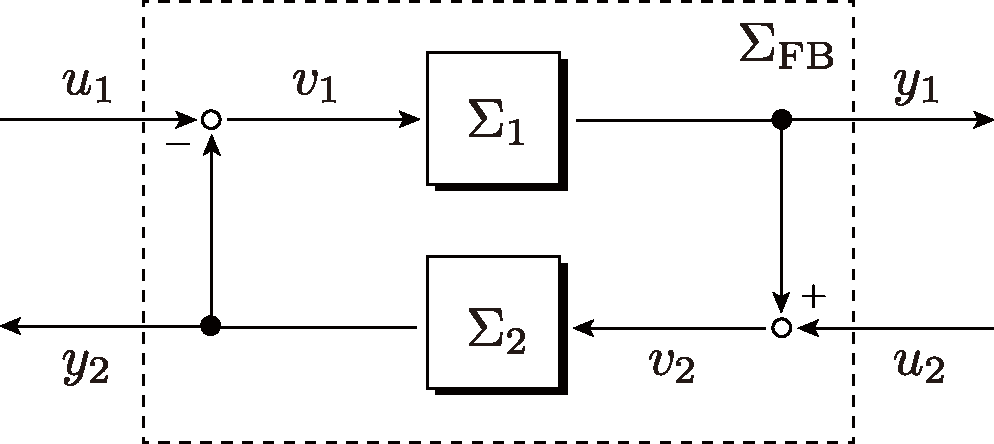
\includegraphics[width = .50\linewidth]{figs/fbnlin}
  \caption{ネガティブ・フィードバック系}
  \label{fig:stasig12}
\end{figure}

\begin{定理}[受動定理]\label{thm:psthm}
\ref{fig:stasig12}に示されるシステム$\Sigma_1$と$\Sigma_2$のネガティブ・フィードバック系$\Sigma_{\rm FB}$を考える。
このとき,$\Sigma_1$が入力$v_1$,出力$y_1$に関して受動的であり,かつ,$\Sigma_2$が入力$v_2$,出力$y_2$に関して受動的であるならば,$\Sigma_{\rm FB}$は入力$(u_1,u_2)$,出力$(y_1,y_2)$に関して受動的である。
特に,$\Sigma_1$が前述の入出力に関して強受動的であるならば,$\Sigma_{\rm FB}$は入力$u_1$,出力$y_1$に関して強受動的である。
さらに,$\Sigma_1$と$\Sigma_2$がどちらも前述の入出力に関して強受動的であるならば,$\Sigma_{\rm FB}$は入力$(u_1,u_2)$,出力$(y_1,y_2)$に関して強受動的である。
\end{定理}

\begin{証明}
まず,$\Sigma_1$と$\Sigma_2$がどちらも強受動的である場合を考える。
システム$\Sigma_i$の入力$v_i$,出力$y_i$に関する蓄積関数を$W_i(x_i)$とする。
このとき,それらの蓄積関数の和に関して
\begin{align*}
\frac{d}{dt}\bigl(W_1(x_1) + W_2(x_2) \bigr) \leq v_1^{\sf T}y_1 + v_2^{\sf T}y_2 
- \rho_1 \|y_1\|^2 - \rho_2 \|y_2\|^2
\end{align*}
が成り立つ。
この不等式に,$v_1=u_1 -y_2$と$v_2=u_2 +y_1$の関係を代入すれば
\begin{align*}
\frac{d}{dt}\bigl(W_1(x_1) + W_2(x_2) \bigr) \leq \mat{u_1^{\sf T} & u_2^{\sf T} }\mat{y_1\\y_2} 
-\rho_{0} 
\left\|
\mat{
y_1\\
y_2
}
\right\|^2
\end{align*}
が得られる。
ただし,$\rho_{0}:=\sfmin \{\rho_1,\rho_2\}$である。
したがって,ネガティブ・フィードバック系の入力$(u_1,u_2)$,出力$(y_1,y_2)$に関する蓄積関数を$W_1(x_1)+W_2(x_2)$と構成できることがわかる。
この議論において,$u_2=0$,$\rho_2=0$とすれば,$\Sigma_1$のみが強受動的である場合の題意が示される。
また,$\rho_1=\rho_2=0$とすれば,$\Sigma_1$と$\Sigma_2$が受動的である場合の題意が示される。
\end{証明}

定理\ref{thm:psthm}の証明に示されているように,フィードバック系の蓄積関数は,結合された2つのシステムの蓄積関数の和として構成することができる。
このように,システムの受動性を示すことができれば,システムが線形であるか非線形であるかを意識することなく,簡潔にフィードバック系の安定性を解析することができる。
なお,結合されるシステムの平衡点が原点である場合には,フィードバック系の平衡点も原点となることは容易に確かめられる。
また,定理\ref{thm:psthm}では,$\Sigma_1$のみが強受動的である場合を考えているが,$\Sigma_2$のみが強受動的である場合も同様である。
3つ以上のシステムが結合される場合にも,同様の解析が可能である\cite{moylan1978stability}。

受動性を用いた安定性解析を行う場合には,「対象とするシステムが受動的か否かを判定すること」が最も重要な課題となる。
そのためには,システムの受動性を示す蓄積関数を構成することが必要である。
しかしながら,特に非線形システムに対しては,構成可能な蓄積関数の形式は一般に明らかではないため,対象とするシステムがもつ物理的な性質などを巧みに利用して,発見的に蓄積関数を見つけ出す必要がある。
なお,電力系統モデルに対しては,発電機の運動エネルギーや電圧のポテンシャルなどから構成されるエネルギー関数が蓄積関数となることが知られている。
このことは,第\ref{sec:psanpw}節で後述する。



\subsection{電力系統モデルの受動性解析}\label{sec:psanpw}

\subsubsection{電力系統モデルの定式化}

本節では,電力系統モデルが平衡点に依らない受動性をもつことを示す。
第\ref{sec:objmod}節で前述したように,送電網は無損失であることを仮定し,式\ref{eq:Ypig}のアドミタンス行列を
\begin{align*}
\bm{Y}=\bm{j}B
\end{align*}
と表す。
このとき,式\ref{eq:ohmY}と式\ref{eq:defPQVIi}の関係を用いれば,バス$i$に機器から供給される有効電力と無効電力は
\begin{align}\label{eq:powbal}
\spliteq{
P_i &= \sum_{j\neq i}^{N} B_{ij} |\bm{V}_i| |\bm{V}_j| \sfsin(\angle \bm{V}_i -\angle \bm{V}_j),
\\
Q_i &= - B_{ii} |\bm{V}_i|^2 -
\sum_{j\neq i}^{N} B_{ij} |\bm{V}_i| |\bm{V}_j| \sfcos(\angle \bm{V}_i -\angle \bm{V}_j)
}
\end{align}
と表せる。
ただし,$B_{ij}$は$B$の$(i,j)$要素を表す。
なお,式\ref{eq:powbal}の等式がすべてのバスで成り立つことは,式\ref{eq:ohmY}の連立方程式が満たされることと等価であることに注意されたい。


発電機が接続されているバスの添字集合を$\mathcal{I}_{\rm G}$と表し,負荷が接続されているバスの添字集合を$\mathcal{I}_{\rm L}$と表す。
ただし,$|\mathcal{I}_{\rm G}| + |\mathcal{I}_{\rm L}| =N$である。
第\ref{sec:objmod}節で前述したように,発電機バスの各$i \in \mathcal{I}_{\rm G}$に対しては
\begin{subequations}\label{eq:modgnld}
\begin{align}\label{eq:modgnlda}
\simode{
\dot{\delta}_i&= \omega_0  \Delta \omega_i\\
M_i   \Delta \dot{\omega}_i&= 
- D_i \Delta\omega_i  
- P_i
+P_{{\rm mech}i}
\\
\tau_{{\rm d}i} \dot{E}_i & = 
 -\frac{X_{{\rm d}i}}{X_{{\rm q}i}}E_i
+\left(
\frac{X_{{\rm d}i}}{X_{{\rm q}i}}-1
\right)
|\bm{V}_i| \sfcos (\delta_i - \angle \bm{V}_i ) 
+ V_{{\rm field}i}
}
\end{align}
の微分方程式に従う発電機モデルが接続されているものとする。
ただし,界磁電圧$V_{{\rm field}i}$は定数であるものとし,各$i \in \mathcal{I}_{\rm G}$に供給される有効電力と無効電力は
\begin{align}\label{eq:modgnldb}
\spliteq{
P_i &= \frac{E_i |\bm{V}_i|}{X_{{\rm q}i}} \sfsin (\delta_i - \angle \bm{V}_i),
\\
Q_i &= \frac{E_i |\bm{V}_i|}{X_{{\rm q}i}} \sfcos (\delta_i - \angle \bm{V}_i)
-\frac{|\bm{V}_i|^2}{X_{{\rm q}i}},
}
\end{align}
である。
また,負荷バスの各$i \in \mathcal{I}_{\rm L}$に対しては
\begin{align}\label{eq:modgnldc}
P_i = P_{{\rm load}i}
,\qquad
Q_i = Q_{{\rm load}i}
\end{align}
\end{subequations}
で表される定電力の負荷モデルが接続されているものとする。
ただし,$P_{{\rm load}i}$と$Q_{{\rm load}i}$は負荷からバスに供給される有効電力と無効電力を表す定数であり,消費を表す場合はそれらの符号は負である。




\subsubsection{受動性に基づく平衡状態の安定性解析}



\begin{定理}[電力系統モデルの平衡点に依らない受動性]\label{thm:nlmain1}
式\ref{eq:powbal}の連立方程式により式(\ref{eq:modgnld})の発電機モデルと負荷モデルが結合された電力系統モデルを考える。
式\ref{eq:alequil}の$\mathcal{E}$により許容可能な平衡点集合を定義する。
このとき,各々すべての$(\Delta \omega^{\star},\delta^{\star},E^{\star}) \in \mathcal{E}$に対して,それらを電力系統モデルの平衡点とする界磁電圧の定常値$V_{\rm field}^{\star}$と機械的トルクの定常値$P_{\rm mech}^{\star}$が存在する。
また,電力系統モデルは,入力$P_{\rm mech}$,出力$\Delta \omega$に関して,平衡点に依らず強受動的である。
\end{定理}

\begin{証明}
式\ref{eq:sys1}の$\mathds{F}$は平衡点に依らず強受動的である。
また,式\ref{eq:sys2}の$\mathds{G}$が平衡点に依らず受動的であることは,その蓄積関数を式\ref{eq:stops}の$W_{(\delta^{\star},E^{\star})}(\delta,E)$に設定することにより示される。
ただし,式\ref{eq:domDf}の$\mathcal{D}$により,その定義域が与えられるものとする。
したがって,定理\ref{thm:eipsthm}から,電力系統モデルは,入力$P_{\rm mech}$,出力$\omega_0 \Delta \omega$に関して平衡点に依らず強受動的である。
さいごに,受動性が出力の正定数倍に関して不変であることから題意が示される。
\end{証明}

定理\ref{thm:nlmain1}では,ある許容可能な平衡点$(\Delta \omega^{\star},\delta^{\star},E^{\star}) \in \mathcal{E}$に対して,それを平衡点とするように,界磁電圧の定常値$V_{\rm field}^{\star}$と機械的トルクの定常値$P_{\rm mech}^{\star}$が設定されていることが暗黙に仮定されていることに注意されたい。
しかしながら,定理\ref{thm:nlmain1}に示されている電力系統モデルの受動性を利用することによって,機械的トルクや界磁電圧を自動的に調整して漸近的に周波数偏差を0とするようなフィードバック制御機構を設計することが可能となる。
このことは第??節で詳述する。

電力系統モデルの漸近安定性に対する結論を述べるため,つぎの用語を導入する。

\begin{定義}[電力系統モデルの平衡状態に関する吸引領域]\label{def:steady}
式\ref{eq:powbal}の連立方程式により式(\ref{eq:modgnld})の発電機モデルと負荷モデルが結合された電力系統モデルを考える。
集合$\mathcal{X}_0$に含まれる任意の初期値に対して,すべての発電機の周波数偏差が漸近的に0となるとき,電力系統モデルは\emph{領域$\mathcal{X}_0$において平衡状態に達する}と呼ぶ。
\end{定義}

定義\ref{def:steady}における領域$\mathcal{X}_0$は,いずれかの許容可能な平衡点に解軌道が漸近的に収束するという意味での\emph{吸引領域}(region of attraction)である。
つぎの定理は,この吸引領域の下からの見積もりを与える。


\begin{定理}[吸引領域の下からの見積もり]\label{thm:nlmain2}
式\ref{eq:powbal}の連立方程式により式(\ref{eq:modgnld})の発電機モデルと負荷モデルが結合された電力系統モデルを考える。
発電機の界磁電圧と機械的トルクが,式\ref{eq:alequil}の許容可能な平衡点集合$\mathcal{E}$のいずれかの点を電力系統モデルの平衡点とするような定数値に設定されているものとする。
このとき,電力系統モデルは領域$\mathbb{R}\times \mathcal{D}$において平衡状態に達する。
ただし,領域$\mathcal{D}$は,式\ref{eq:domDf}により定義される。
\end{定理}


\begin{証明}
補題\ref{lem:eipssta}を用いて各々すべての平衡点の漸近安定性を示すためには,式\ref{eq:eizeroso}で示される平衡状態の可観測性を示せば良い。
ただし,電力系統モデルには,すべての発電機の回転子偏角を同じ値だけ変化させるような,本質的に等価な平衡点の集合が存在するため,それらの平衡点における解軌道はすべて同一視するような可観測性を考える必要がある。
具体的には,ある$(\delta^{\star},E^{\star}) \in \mathcal{E}_{\mathds{G}}$を平衡点とする$V_{\rm field}^{\star}$を考えると,任意の定数$c$に対して$(\delta^{\star}+c \mathds{1},E^{\star}) \in \mathcal{E}_{\mathds{G}}$は同じ$V_{\rm field}^{\star}$により平衡点となる。
このことは,ある$\delta^{\star}+c \mathds{1}$に対して,必ず$\angle \bm{V}^{\star}+c \mathds{1}$が存在し,式(\ref{eq:eqeq})が満たされることから確認できる。
この本質的に等価な平衡点の集合を$(\delta^{\star} ,E^{\star})_{\rm eq} \subseteq \mathcal{E}_{\mathds{G}}$と表す。

まず,式\ref{eq:modgnlda}の$\Delta \omega$に関する微分方程式に注目する。
電力系統モデルの出力は状態$\Delta \omega$に等しいことから,
入力が恒等的に$P_{\rm mech}^{\star}$であるとき,出力が恒等的に$\Delta \omega^{\star}=0$となるような解軌道は,明らかに$\Delta \omega(t) = \Delta \omega^{\star}$のみである。
このとき,必ず$P = P_{\rm mech}^{\star}$である。
したがって,題意を示すためには,式\ref{eq:sys2}の$\mathds{G}$の出力が恒等的に$y_{\mathds{G}}^{\star} = P_{\rm mech}^{\star}$であるときに,
$\mathds{G}$の平衡点集合$(\delta^{\star} ,E^{\star})_{\rm eq}$が唯一に特定できることを示せば良い。

この事実は以下のように示される。
まず,式\ref{eq:potWx}の$U_{\mathds{G}}(\delta, E; |\bm{V}|, \angle \bm{V})$がすべての引数に関して微分可能であることから,式\ref{eq:stops0}の$W(\delta,E)$は滑らかな関数であることがわかる。
したがって,その勾配関数$\nabla W(\delta,E)$は一価関数である。
また,補題\ref{lem:volpot}の証明における偏微分の計算から,式(\ref{eq:eqeq})の連立方程式は
\begin{align}\label{eq:nabeqW}
\nabla W(\delta^{\star},E^{\star})
=
\mat{
P_{\rm mech}^{\star} \\
\sfdiag\left(\frac{1}{X_{{\rm d}i} - X_{{\rm q}i}}\right) V_{\rm field}^{\star}
}
\end{align}
に等しいことがわかる。
いま,式\ref{eq:domDf}の定義から,$W(\delta,E)$は領域$\mathcal{D}$において凸関数であるため,$\nabla W(\delta,E)$は領域$\mathcal{D}$において単調増加関数である\cite{rockafellar1970convex,boyd2004convex}。
したがって,式\ref{eq:nabeqW}の方程式は,解が存在するのであればそれは一意である。
以上より,$V_{\rm field}^{\star}$がある定数として与えられ,さらに,出力の定常値$y_{\mathds{G}}^{\star}$が指定されるのであれば,その平衡点集合$(\delta^{\star} ,E^{\star})_{\rm eq}$が領域$\mathcal{D}$において唯一に特定されることがわかる。

さいごに,$\mathcal{E}$に含まれる各々の平衡点の吸引領域が$\mathbb{R}\times \mathcal{D}$であることは,式\ref{eq:sys1}の$\mathds{F}$の受動性を示す蓄積関数
\begin{align*}
W_{\Delta \omega^{\star}}(\Delta \omega)= \frac{\omega_0}{2}
(\Delta \omega -\Delta \omega^{\star})^{\sf T}
\sfdiag(M_i)
(\Delta \omega -\Delta \omega^{\star})
\end{align*}
の定義域が$\mathbb{R}$であることと,式\ref{eq:sys2}の$\mathds{G}$の蓄積関数の定義域が$\mathcal{D}$であることから示される。
\end{証明}

定理\ref{thm:nlmain2}では,発電機の物理パラメータに関する条件は何も課されていないことに注目すると,領域$\mathbb{R}\times \mathcal{D}$は,すべての発電機の物理パラメータに対して,いずれかの許容可能な平衡点に電力系統モデルの解軌道が漸近的に収束するような吸引領域であることがわかる。
一般に,受動性に基づく解析では,漸近安定性に対する十分条件が与えられるだけであるため,この吸引領域$\mathbb{R}\times \mathcal{D}$は,最大の吸引領域よりも保守的な見積もりとなる。
すなわち,すべての発電機の物理パラメータに対して,いずれかの許容可能な平衡点に電力系統モデルの解軌道が漸近的に収束するような「最大」の吸引領域を$\mathbb{R}\times\mathcal{D}_{\sfmax}$と表せば,
$\mathcal{D} \subseteq \mathcal{D}_{\sfmax}$
の包含関係が必ず成り立つ。

以下では,第\ref{sec:stalin}節における近似線形モデルの漸近安定性解析の結果に基づいて,
%領域$\mathcal{D}$による最大の吸引領域$\mathcal{D}_{\sfmax}$の保守亭について
これら$\mathcal{D}$と$\mathcal{D}_{\sfmax}$の間にどの程度の乖離があるのかを考察する。
式\ref{eq:Wpd}の不等式で表されているように,領域$\mathcal{D}$は関数$W(\delta,E)$が凸関数となるような領域である。
この関数$W(\delta,E)$の凸性は,ヘッセ行列$\nabla^2 W(\delta,E)$の正定性により特徴づけられる(\red{付録??})。
具体的には
\begin{align}\label{eq:domDpl}
\mathcal{D}_{+}:= \left\{
(\delta, E) \in \mathbb{R}^{2 |\mathcal{I}_{\rm G}|}  :
\nabla^2 W(\delta,E) \succeq 0
\right\}
\end{align}
と表すことができる。
ただし,この定義における領域$\mathcal{D}_{+}$は,領域$\mathcal{D}$と厳密に一致するとは限らず,一般には$\mathcal{D} \subseteq \mathcal{D}_{+}$となる領域である。
その理由は,式\ref{eq:Wpd}の不等式では,平衡点を除く領域で$W(\delta,E)$が狭義凸関数となることを条件として課しているのに対して,式\ref{eq:domDpl}では弱い意味での凸性を条件として課しているためである。
なお,式\ref{eq:domDpl}の半正定性の条件を単純に正定性に強めることはできない。
その理由は後述する。

つぎの定理は,\red{各々すべてのバスに発電機モデルが接続されている場合に,}領域$\mathcal{D}^+$に対して有用な解釈を与える。


\begin{定理}[ポテンシャル関数のヘッセ行列と近似線形モデルの関係]
\label{thm:hess}
式\ref{eq:powbal}の連立方程式により式\ref{eq:modgnlda}の発電機モデルが結合された電力系統モデルを考える。
また,式\ref{eq:sysmats}により,$(\delta^{\star}, E^{\star})$の関数として行列$A$,$B$,$C$,$L$を定義する。
式\ref{eq:stops0}の関数$W(\delta, E)$に対するヘッセ行列を
\begin{align*}
\nabla^2 W(\delta, E)
=
\mat{
\nabla^2_{\delta} W (\delta, E) & \nabla^2_{\delta,E} W(\delta, E)\\
\nabla^2_{E,\delta} W (\delta, E) & \nabla^2_{E} W (\delta, E)
}
\end{align*}
と表すとき,$\nabla^2_{E} W(\delta^{\star}, E^{\star})$が正定であることは,$A$が安定であることと等価である。
特に,$A$が安定であるとき,$\nabla^2 W(\delta^{\star}, E^{\star})$が半正定であることは,$L-CA^{-1}B$が半正定であることと等価である。
\end{定理}

\begin{証明}
要素が$M_{ij}$である行列$M$を$[M_{ij}]_{ij}$と表す。
まず,式\ref{eq:sysmats}の行列$A$について考える。
式\ref{eq:lindyn}の近似線形モデルの微分方程式から,$A$は内部電圧$E$の時間微分がそれ自身に依存する項を表すシステム行列であることがわかる。
すなわち
\begin{align*}
A = \left[
\left.
\frac{\partial}{\partial E_j}
\left\{
-\frac{X_{{\rm d}i}}{X_{{\rm q}i}}E_i
+\left(
\frac{X_{{\rm d}i}}{X_{{\rm q}i}}-1
\right)
|\bm{V}_i| \sfcos (\delta_i - \angle \bm{V}_i ) 
\right\}
\right|_{(\delta,E)=(\delta^{\star},E^{\star})}
\right]_{ij}
\end{align*}
である。
ただし,$(|\bm{V}|,\angle \bm{V})$には式\ref{eq:eqeqa}を満たす$(|\bm{V}^{\star}|,\angle \bm{V}^{\star})$を代入するものとする。
一方で,補題\ref{lem:volpot}の結果を用いると
\begin{align*}
&\left[
\left.
\frac{\partial}{\partial E_j}
\frac{\partial W}{\partial E_i}
\right|_{(\delta,E)=(\delta^{\star},E^{\star})}
\right]_{ij}
=
\Biggl[
\Biggl.
-\frac{1}{X_{{\rm d}i} - X_{{\rm q}i}}
\frac{\partial}{\partial E_i}
\Biggl\{
-\frac{X_{{\rm d}i}}{X_{{\rm q}i}}E_i
\\
&\hspace{10em}
+\left(
\frac{X_{{\rm d}i}}{X_{{\rm q}i}}-1
\right)
|\bm{V}_i| \sfcos (\delta_i - \angle \bm{V}_i ) 
\Biggr\}
\Biggr|_{(\delta,E)=(\delta^{\star},E^{\star})}
\Biggr]_{ij}
\end{align*}
が得られる。
したがって,
\begin{align*}
\nabla^2_{E} W(\delta^{\star}, E^{\star})
= 
-\sfdiag\left(
\frac{1}{X_{{\rm d}i} - X_{{\rm q}i}}
\right)
A
\end{align*}
であることから,$\nabla^2_{E} W(\delta^{\star}, E^{\star})$の正定性と$A$の安定性は等価であることがわかる。
同様に,
\begin{align*}
\nabla^2_{\delta,E} W(\delta^{\star}, E^{\star})
&=
-\sfdiag\left(
\frac{1}{X_{{\rm d}i} - X_{{\rm q}i}}
\right)
B,
\qquad
\nabla^2_{\delta} W(\delta^{\star}, E^{\star})
=L
\\
\nabla^2_{E,\delta} W(\delta^{\star}, E^{\star})
& =
C
\end{align*}
であることがわかる。
したがって,$A$が安定であるとき,すなわち,$\nabla^2_{E} W(\delta^{\star}, E^{\star})$が正定であるとき,シューア補行列の性質から,$\nabla^2 W(\delta^{\star}, E^{\star})$が半正定であることは,$L-CA^{-1}B$が半正定であることと等価である。
\end{証明}

定理\ref{thm:EdynNI}に示されているように,送電網が無損失である場合には,$L-CA^{-1}B$が半正定であることが,式\ref{eq:trGs}の伝達関数$G(s)$が正実となるための必要条件となっている。
定理\ref{thm:hess}に基づいて言い換えれば,式\ref{eq:domDpl}の領域$\mathcal{D}_{+}$の内部で近似線形モデルを導出することが,そのシステムが受動的となるための必要条件である。
この事実は,本節における非線形システムの解析結果と符合している。
すなわち,式\ref{eq:sys2}の$\mathds{G}$の蓄積関数の定義域は$\mathcal{D}\subseteq \mathcal{D}_{+}$となっている。

また,定理\ref{thm:sync}に示されているように,$L-CA^{-1}B$の半正定性は,すべての発電機の物理パラメータに対して近似線形モデルが漸近安定となるための必要条件になっている。
したがって,定理\ref{thm:hess}の等価性から,式\ref{eq:domDpl}の領域$\mathcal{D}_{+}$は,最大の吸引領域$\mathcal{D}_{\sfmax}$を包含する領域であることがわかる。
以上の議論により
\begin{align}\label{eq:setinv}
\mathcal{D} \subseteq \mathcal{D}_{\sfmax} \subseteq \mathcal{D}_{+}
\end{align}
の包含関係が導かれる。
前述のように,領域$\mathcal{D}$は平衡点を除く領域で$W(\delta,E)$が狭義凸関数となるように定義されているのに対して,領域$\mathcal{D}_{+}$は$W(\delta,E)$が弱い意味で凸関数となるように定義されている。
これは,$\mathcal{D}$と$\mathcal{D}_{+}$の差は,不等式の等号を含めるか否かだけの差であることを意味している。
しがたって,固有値の変化がパラメータ変化に関して連続的であることを考えると,式\ref{eq:setinv}の3つの領域は本質的に同等であることが結論づけられる。
これらの事実から,非線形システムに対する最大の吸引領域$\mathcal{D}_{\sfmax}$が,近似線形モデルに関する$L-CA^{-1}B$の正定性により特徴づけられることがわかる。
なお,$L-CA^{-1}B$は必ず零固有値をもつことから,ヘッセ行列$\nabla^2 W(\delta,E)$は狭義の正定行列にはならないため,式\ref{eq:domDpl}の行列不等式を等号を含めない不等式に単純に換えることはできない。

一般に,あるシステムの受動性が特定の蓄積関数に対して示されたとしても,それ以外に可能な蓄積関数が存在するか否かは自明ではない。
したがって,非線形システムの最大の吸引領域$\mathcal{D}_{\sfmax}$が,式\ref{eq:stops}の蓄積関数を用いた受動性の議論だけから導かれるという事実は興味深いものである。
この意味で,\ref{lem:volpot}のポテンシャル関数は,物理的にも数学的にも電力系統モデルの本質的な特徴を捉えたものであることが示唆される。


\section{同期安定化制御}
\subsection{系統安定化装置と自動電圧調整器}
\subsection{同期安定化制御の数値シミュレーション}
\subsection{レトロフィット制御理論に基づく同期安定化制御\advanced}


\newpage
%\printindex
%
%
\end{document}